We now show how to apply the learning bias of \autoref{sec:new_bias} on undirected graphs.
Furthermore, we assume that the strong balance holds, meaning that there are only two groups
according to \autoref{thm:structural}. In other words, the labelling of $E$ is consistent with a
two-clustering of $V$. Namely, $V$ can be partitioned in two clusters such that edges within each
cluster are positive and edges across clusters are negative.
In that case, the following
\emph{multiplicative rule} holds: for any nodes $u$, $v$ in $V$, and any path $p$ between $u$ and
$v$ in $G$, the sign $\yuv$ is equal to the product of the signs along $p$. Hereafter, we call this
product the parity of $p$, and denote it by $\pi(p)$.
While it is a simple and convenient hypothesis, this is too strong
of a requirement to be satisfied in practice. Therefore, we relax it by assuming that, starting from
a consistent labeling $Y$, we can only observe a randomly perturbed version $Y'$ of $Y$.
Specifically, given a constant $q\in [0, \nicefrac{1}{2})$, every sign of $Y$ is flipped with a
probability smaller than $q$. We denote by $E_{\mathrm{flip}} \subset E$ the set of edges whose sign
has been flipped.

In this section, we are interested in active learning algorithms that first query a subset
$\etrain$ of the edges, observe the signs in $\etrain$ and use them to predict the remaining signs.
More precisely, we focus on an algorithm that queries a spanning tree $T$ of $G$ and predicts the
sign of an edge $(u,v) \in \etest = E \setminus E_T$ as the parity of $\pathtuv$. Intuitively, since
each sign has been potentially flipped, the longer the path in $T$, the more likely its parity will
be not be equal to the true sign $\yuv{}$. Therefore we would like each such path to be as short as
possible.
Formally, the number of mistakes of such an algorithm is upper bounded by~\autocite[Equation
(3)]{Cesa-Bianchi2012b}
\begin{equation*}
  |E_{\mathrm{flip}}| + \sum_{(u,v) \in \etest}
  \sum_{e\in E} \Ind{e \in \pathtuv} \Ind{e \in E_{\mathrm{flip}}}
\end{equation*}
which in expectation is equal to:
\begin{equation}
  \label{eq:stretch_mistakes}
  q\left(|E| + \sum_{(u,v) \in \etest} |\pathtuv| \right)
\end{equation}
In the following, we describe a way to build spanning trees tailored for this situation. More
precisely, we implement and analyze a suggestion made to us by~\autocite{gtxFabio}.

\subsection{\gtx{}: a spanning tree designed for sign prediction}
\label{sub:gtx_algo}

To achieve our objective of building a spanning tree that minimizes the distances between all
connected pair of nodes in the original graph, we rely on a particular subgraph structure, namely
the star.  We therefore introduce two algorithmic primitives: \extractStar{}, which partition a
graph $G$ into a set of disjoint stars; and \collapseStar{}, which selects edges from $E$ to
assemble these stars into a new, smaller graph. Given a graph topology $G_0=(V_0, E_0)$ and assuming
for simplicity that $G_0$ consists of a single connected component,\footnote{For we can otherwise
run our algorithm in parallel on each connected components of $G_0$.} the \gtx{} algorithm
repeatedly applies these two primitives to produce a sequence of graphs $\{G_t\}_{t=0}^K$ of
decreasing size, until $G_K$ is made of a single node. All the edges selected while reaching
this stage then form the spanning tree we were looking for.
% [from a CMU NIPS submission http://www.stat.cmu.edu/~arinaldo/papers/mutualfriends.pdf] We
% consider Mutual-Friends to be *an algorithmic primitive*, by which we mean a kind of subroutine for
% a more complicated function that iterates Mutual-Friends, similarly to [5].

In the following, we provide a more precise description of our two primitives and analyze their
complexity. Then we state formally the complete \gtx{} algorithm, prove its termination and
correctness, and show a detailed example of its execution.  Finally, we study its properties, such
as the number of iterations needed to finish and the stretch of the resulting tree.

\paragraph{\extractStar{}}\label{par:extractstar}%
\extractStar{} takes as input a graph $G_t=(V_t, E_t)$.
While the nodeset $V_t$ is not exhausted, it repeatedly samples a
node $c_i$, creates a star $S_i^t$ with $c_i$ at its center and the neighbors of $c_i$ on the
periphery, removes all the nodes of $S_i^t$ from
$V_t$ and all the edges incident to $S_i^t$ from $E_t$, and finally decrements accordingly the
degree of the 2-hop neighbors of $c_i$ (see \autoref{fig:gtx_star_simple} for a visual
representation of this notation).
Upon completion, it returns a list of stars,
the set of all the edges within a star,
and a map (or associative array) that associates each node of $V_t$ to the index of the
unique star it belongs to.
According to the definition of \textcite{HashTableBook08}, an associative array is an abstract data
type composed of a collection of (key, value) pairs, such that each possible key appears at most
once in the collection. It efficiently supports the addition, removal and modification of a pair, as
well as the lookup of a value associated with a particular key.
\begin{marginfigure}
  \centering
  \includegraphics[height=0.15\textheight]{assets/tikz/gtx_star_tikz.pdf}
  \caption[A sample star]{A sample star created during the \tth{} collapse level. The black node
    % \tikz{\node[vertex,rare] {$c_i$};}
    is the center $c_i$ of the star $S_i^t$, which is also made of the four light gray peripheral nodes
  % \tikz{\node[vertex,medium] {$p_1$};} to \tikz{\node[vertex,medium] {$p_4$};}
  as well as the solid edges. The 2-hops neighbors of $c_i$ are the white nodes
  % \tikz{\node[vertex] {$h_1$};} to \tikz{\node[vertex] {$h_3$};}
  $h_1$ to $h_3$, whose degree will decrease once $S_i^t$ is removed from $G_t$.}
  \label{fig:gtx_star_simple}
\end{marginfigure}

As showed in the following pseudo code\footnote{Note that for
clarity, we removed some bookkeeping code in all listings, mainly the part related to maintaining
mapping between nodes at different collapse level. However, the full python implementation
is available at \url{https://github.com/daureg/magnet/blob/master/veverica/new_galaxy.py\#L27}.}, we
sample centers by choosing the node with the current highest degree, with ties broken
arbitrarily.\footnote{We also consider more involved heuristics but, in the interest of simplicity,
they are presented later~\vpageref{ssec:gtx_center_choice}.} This is achieved efficiently by
maintaining a max-priority queue $Q$, initially containing all the nodes of $V_t$. The priority of a
node is its current degree and we equip $Q$ with two standard operations described
by~\textcite[section 6.5]{CormenAlgo09}: \textsc{Extract-Max}$(Q)$ removes and returns the
node of $Q$ with the largest degree and \textsc{Decrease-Key}$(Q$, $u$, $\Delta)$ decrements
the degree of the node $u$ by an amount $\Delta$.
We also assume that $G$ is the adjacency list of the graph, so that $G[u]$ is the set of neighbors of
$u$, \ie{} $G[u] \equiv \mathcal{N}(u)$. Finally $membership$ is a map and we
define the \textsc{Star} function, which creates a star given a center $c$, a list $periphery$ of
peripheral nodes, and a star index $i$. After creating the \ith{} star, for every node $u$ belonging
to that star, the \textsc{Star} function sets $membership[u] = i$.
\vspace{-\baselineskip}

\begin{center}
  \rule{\textwidth}{.3pt}
  \begin{algorithmic}[1]
    \Function{\extractStar{}}{$G_t=(V_t,E_t)$}
      \State Let $Q$ be the max-priority queue described above
      \State Let $remaining$ be a set of nodes, initially containing all the nodes in $V_t$
      \State Let $membership$ be an empty map
      \Let{$stars$}{$[]$}
      \Let{$inner\_edges$}{$\emptyset$}
      \While{$Q$ is not empty}
        \Let{$c$}{\Call{Extract-Max}{$Q$}}
        \If{$c$ not in $remaining$}
          \State \textbf{continue} \Comment{$c$ is part of an existing star so there is
          nothing to do}
        \EndIf
        \Let{$periphery$}{$G_t[c] \bigcap remaining$}
        \Let{$stars$}{$stars \bigcup \{$\Call{Star}{$c$, $periphery$, $|stars|$}\}}
        \Let{$inner\_edges$}{$inner\_edges \bigcup \{(c, p): p \in periphery\}$}
        \Let{$remaining$}{$remaining \setminus \left\{ \{c_i\} \cup periphery\right\}$}
        \For{$p$ in $periphery$}
          \For{$h$ in $G_t[p] \bigcap remaining$}
            \State \Call{Decrease-Key}{$Q$, $h$, $1$}
          \EndFor
        \EndFor
      \EndWhile
      \State \textbf{return} $stars$, $inner\_edges$, $membership$
    \EndFunction
  \end{algorithmic}
  \rule{\textwidth}{.3pt}
\end{center}

\begin{prop}
  \label{prop:gtx_time_extractstar}
  For any connected graph $G=(V,E)$, \extractStar$(G)$ terminates in $O(|E|)$ time.
\end{prop}
\begin{proof}
\extractStar{} terminates because at each iteration of the while loop line 7, we remove one node
from $Q$ and never add any. Let us now analyze its complexity. We first build a priority queue of
all the nodes according to their degree (line 2), which requires $|V|$ insertions into $Q$. Then
we execute $|V|$ iterations of the while loop. However, the main idea here is that we process each
node and each edge exactly once. We first find the center $c$ of the next star by extracting the
maximum of the queue (line 8) and testing if $c$ is still part of the graph, which happens $|V|$
time. Then we build the corresponding star (line 11--14). In total, we test the membership of $|V|$
nodes in line 11, $\textsc{Star}$ updates the $membership$ map $|V|$ times in line 12,
$inner\_edges$ consists of $|E|$ edges at most in line 13 and $remaining$ is only updated $|V|$
times in line 14. Finally, we decrease the priority (\ie{} the degree) of all nodes adjacent to the
new star (line 15--17). Each decrement is supported by a single edge, thus \textsc{Decrease-Keys} is
called at most $|E|$ times. Since all queue operations require constant time when using a Strict
Fibonacci Heap~\autocite{FibonacciHeaps12}, the complexity is $O(|E|+|V|)$, which is also $O(|E|)$
since $G$ is connected.
\end{proof}

\paragraph{\collapseStar{}}\label{par:collapsestar}%

The second primitive, \collapseStar{} takes as input the edges $E_t$ of the current graph, along
with the $membership$ result of \extractStar{} and an $eccentricity$ array. It builds a new graph
$G_{t+1}$ where each star from \extractStar{} becomes a node and where there is a link between two
nodes $s_u$ and $s_v$ if the nodes in $V_t$ making up $s_u$ and $s_v$ are connected in $E_t$. The
$eccentricity$ array is needed because when connecting two stars, we would prefer to join their
center rather than two of their peripheral points. Therefore, we maintain an eccentricity count for
all of the nodes of the original $G_0$, which is incremented by $1$ each time a node is chosen to be
on the periphery of a star. In other words, the eccentricity of an original node quantifies to which
extent it has been pushed to the border of the galaxy.

\begin{marginfigure}
  \centering
  \includegraphics[width=0.92\linewidth]{assets/tikz/gtx_cross_edges_tikz.pdf}
  \caption[Cross edge representation]{In this graph, there are four possible edges between the two
  stars $s_1$ and $s_2$, and all are part of $cross\_edges[(s_1, s_2)]$, here represented in light
red. Those edges are labeled with the sum of eccentricity of their underlying endpoints, and the
minimal one is linking a peripheral node of $s_1$ directly to the center of $s_2$.}
  \label{fig:gtx_cross_edge}
\end{marginfigure}%
\collapseStar{} not only returns the new graph $G_{t+1}$ but also a map $cross\_edges$. This map is
used to keep track of which edge in $E_t$ connects any pair of node in $V_{t+1}$ (as illustrated in
\autoref{fig:gtx_cross_edge}). It associates to any edge in $E_{t+1}$ a set of edges from $E_t$.
This set can have an arbitrary size during the execution of \collapseStar{}, yet it is guaranteed to
contain a single edge upon termination. Although this does not appear in the following pseudo code,
in practice we ensure that $(s_u, s_v)$ and $(s_v, s_u)$ refer to the same edge in $cross\_edges$.

\begin{center}
  \rule{\textwidth}{.3pt}
  \begin{algorithmic}[1]
    \Function{\collapseStar{}}{$E_t,\,membership,\,eccentricity$}
      \State Let $G_{t+1}$ be an empty graph
      \State Let $cross\_edges$ be the map described above
      \ForAll{edge $(u, v)$ in $E_t$}
      \Let{$s_u$}{$membership[u]$}
      \Let{$s_v$}{$membership[v]$}
        \If{$u$ and $v$ are not in the same star (\ie{} $s_u \neq s_v$)}
          \Let{$cross\_edges[(s_u, s_v)]$}{$cross\_edges[(s_u, s_v)] \bigcup \{(u, v)\}$}
        \EndIf
      \EndFor
      \ForAll{pair of will-be connected stars $(s_u,s_v)$ in $cross\_edges$}
        \Let{$possible\_underlying\_edges$}{$cross\_edges[(s_u, s_v)]$}
        \marginpars{\small Line 11 is actually a simplification since the $eccentricity$ array is only
        defined for nodes in $V_0$ so when \collapseStar{} is called on $G_3$ for instance, $u$ and $v$
        are nodes of $V_3$ and we have to retrieve the actual corresponding edge in $E_0$. Maybe I could
        simply add a map from $E_t$ to $E_0$ like in the real python code…}
        \State $$(u_0, v_0) \gets \argmin_{(u,v)\in possible\_underlying\_edges} eccentricity[u]+eccentricity[v]$$
        \Let{$cross\_edges[(s_u, s_v)]$}{$\{(u_0, v_0)\}$}
        \Let{$E_{t+1}$}{$E_{t+1} \bigcup \{(s_u, s_v)\}$}
      \EndFor
      \State \textbf{return} $G_{t+1}$, $cross\_edges$
    \EndFunction
  \end{algorithmic}
  \rule{\textwidth}{.3pt}
\end{center}

\begin{prop}
  \label{prop:gtx_time_collapsestar}
  For any graph $G=(V,E)$, \collapseStar$(E$, $membership$, $eccentricity)$ terminates in $O(|E|)$
  time.
\end{prop}
\begin{proof}
  The analysis of \collapseStar{} is rather straightforward because the function only executes two
  loops over $E$. During the for loop of line 4, it only performs constant time
  operations on maps. Likewise, in the for loop of line 9, the most expensive operation is finding the minimum
  in line 11. Computing the eccentricity of an edge is done in constant time and only once for each
  edge of $E$.  As a consequence, the total time of \collapseStar{} is indeed $O(|E|)$.
\end{proof}

\paragraph{Putting the pieces together}\label{par:full_gtx}%
\extractStar{} and \collapseStar{} are truly the core the of \gtx{} algorithm but to obtain our
final spanning tree, we need additional work, namely updating the eccentricity of the nodes of
$V_0$ and keeping track of each edge within and between stars along every collapse steps. Despite
our earlier promise, this entails showing some bookkeeping code, because it has an influence on the
runtime of \gtx{}. \Todo{Those maps could probably use better names}
Namely in the listing of \autoref{alg:gtx} \vpageref{alg:gtx}, we use the three following maps:

\vspace{0.5\baselineskip}
\noindent\begin{tabulary}{187mm}{lllL}
  \toprule
  name               & keys set at $t$ & values set at $t$   & comment \\
  \midrule
  $star\_membership$ & nodes in $V_t$  & nodes in $V_{t+1}$  & this is the map returned by
  \extractStar{}$(G_t)$ \\
  $full\_membership$ & nodes in $V_0$  & nodes in $V_{t+1}$  & at $t=0$, this is equals to
  $star\_membership$ and then it gets updated at every iteration to maintain its original keys set.  \\
  $original\_node$   & nodes in $V_t$  & sets of $V_0$ nodes & This can be seen as the reverse of
  $full\_membership$ and it is the one needed to update the eccentricity of the original nodes. \\
  \bottomrule
\end{tabulary}
\vspace{0.5\baselineskip}

\begin{algorithm}[tbh]
  \caption{\gtx{}($G_0=(V_0,E_0)$) \label{alg:gtx}}
	\begin{algorithmic}[1]
    \State Let $eccentricity$ be an array of size $|V_0|$ initially all set to $0$
    \Let{$G_t$}{$G_0$}
    \Let{$inner\_edges\_seq$, $outer\_edges\_seq$}{$[]$, $[]$}
    \Repeat
      \Let{$stars$, $inner\_edges$, $membership$}{\Call{Extract-Stars}{$G_t$}}
      \State Add $inner\_edges$ to the list $inner\_edges\_seq$
      \State \Call{Update-Eccentricity}{$stars$, $eccentricity$, $original\_node$}
      \Let{$full\_membership$, $original\_node$}{\Call{Update-Nodes-Mapping}{$full\_membership$, $membership$}}
      \Let{$G_{t+1}$, $\!outer\_edges$}{\Call{Collapse-Stars}{$E_t \!\setminus\! inner\_edges$,
      $\!membership$, $\!eccentricity$}}
      \State Add $outer\_edges$ to the list $outer\_edges\_seq$
      \Let{$G_{t}$}{$G_{t+1}$}
    \Until{$|outer\_edges|>0$}
    \State \textbf{return} \Call{Assemble-Spanning-Tree}{$inner\_edges\_seq$, $outer\_edges\_seq$}
		\begin{center}
      \vspace{-.5\baselineskip}
			\rule{0.5\textwidth}{.2pt}
		\end{center}
    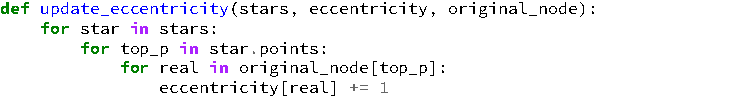
\includegraphics{assets/tmp-code/update_eccentricity.pdf}
    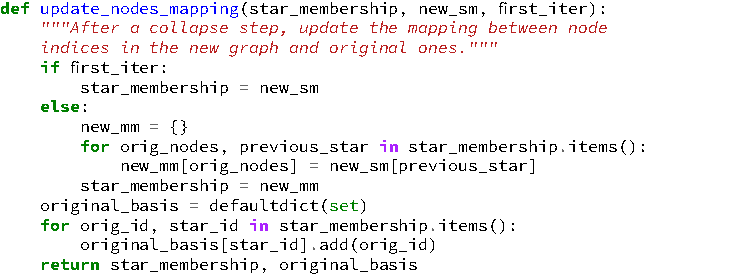
\includegraphics{assets/tmp-code/update_nodes_mapping.pdf}
    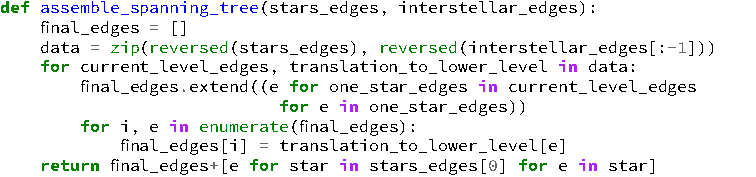
\includegraphics{assets/tmp-code/assemble_spanning_tree.pdf}
	\end{algorithmic}
\end{algorithm}

As described in \autoref{alg:gtx}, at every collapse level, we first extract stars from the current
graph (line 5), then update the eccentricity and node mappings (lines 7--8) and finally collapse the
graph (line 9). We perform these operations until there are no edge connecting stars anymore. At
this point, we revisit every outer edges to build the spanning tree (line 13).

\begin{prop}
  \label{prop:gtx_correct}
  For any connected graph $G_0$, \gtx$(G_0)$ terminates after $K\leq |V_0|$ iterations. Furthermore,
  it runs in $O(K|E_0|)$ time and returns a spanning tree of $G_0$.
\end{prop}
We will need the following lemma.
\begin{lemma}
  \label{lem:gtx_stay_connected}
  If $G_0$ is connected, then any subsequent graph $G_t,\, t \leq K$ is also connected.
\end{lemma}
\begin{proof}
 Suppose not and assume, to the contrary, that there exists at least one (or more) disconnected
 graph in $\{G_t\}_{t=1}^K$ and let $t_0$ be the smallest index such that $G_{t_0}$ is disconnected.
 Then there exist two nodes $s_u$ and $s_v$ in $V_{t_0}$ with no path between them in $E_{t_0}$.
 Letting $\mathcal{U}, \mathcal{V} \subset V_{t_0-1}$ be respectively the nodes forming stars $u$
 and $v$, this implies there is no path between nodes in $\mathcal{U}$ and nodes in $\mathcal{V}$.
 However, $G_{t_0-1}$ is connected by hypothesis, which leads to a contradiction.
\end{proof}

\begin{proof}[Proof of \autoref{prop:gtx_correct}]
  Let us first show that \gtx{} terminates in less than $|V_0|$ iterations. This follows from the
  fact that every time we collapse the graph $G_t$, we strictly reduce the number of nodes. Indeed,
  according to \autoref{lem:gtx_stay_connected}, $G_t$ is connected so at least two nodes of $V_t$
  are joined by an edge and will form a star, \ie{} a single node. We can thus claim that $|V_{t+1}| <
  |V_t|$. Note also that for all $t$, $|V_t| > 0$ and that when $|V_t|=1$, \extractStar{} creates a
  singleton and \collapseStar{} does not return any outer edges so \gtx{} finishes, proving that the
  number of iterations $K$ satisfies $K \leq |V_0|$.

 Then we analyze the time complexity. We already now that during the \tth{} iteration,
 \extractStar{} and \collapseStar{} take time $O(|E_t|)$. We provide only the actual python code
 instead of pseudo code for the remaining functions since they do not present any special
 interesting algorithmic aspect. However, we can say that \textsc{Update-Eccentricity} and
 \textsc{Update-Nodes-Mapping} take $O(|V_0|)$ time since they go through every node of the original
 graph. Because $G_0$ is connected, $|V_0| \leq |E_0|$, and since for all $t$, $|E_t| \leq |E_0|$,
 we have that the \gtx{} inner loop takes $O(K|E_0|)$ time. Finally, since
 \textsc{assemble-spanning-tree} goes again through every edge visited at every collapse step, it
 also takes $O(K|E_0|)$ time, which is thus the overall complexity of the \gtx{} algorithm.

  Finally we prove that \gtx{} indeed returns a spanning tree of $G_0$.
\end{proof}


Later we hope to found an upper bound of $T$ in terms of $m$, and also to refine the analysis to
leverage the fact that $\sum_{t=0}^T |E_t|$ is significantly smaller than $Tm$. For now, let us
prove the termination of \gtx{} by observing that, assuming $|E_t|>0$, $|E_{t+1}| < |E_t|$ since
at least two nodes in $G_t$ are connected and will therefore form a star, which will remove all the
inner edges of that star. As for the fact that we get a tree, note that a star is a tree, therefore
a star of star is a tree, and so on.\Todo{make the two arguments about \gtx{} correctness more
formal, and also explain that since all nodes are part of the ultimate star, this tree is a spanning
one. Motivate the name of \gtx{}.}

\paragraph{Example of \gtx{}}
\label{par:exemple_of_gtx}

We illustrate the operation of the \gtx{} algorithm on a small (and somewhat contrived) example.
Let us start with the initial graph $G_0$ depicted in \autoref{fig:gtx_eccentricity}
\vpageref{fig:gtx_eccentricity} and initialize
the eccentricity of all nodes to $0$. When running \extractStar{}, we see that the maximum degree is
$4$, achieved at nodes $\{1, 6, 11, 16, 21, 26, 31, 36, 41\}$. For the sake of simplicity, assume
nodes are picked according to their index. First, node $1$ forms the star $\starone{1}$ with
peripheral nodes $2$, $3$, $4$ and $5$. This increments the eccentricity of those peripheral nodes
by $1$. Then node $6$ forms its star $\starone{2}$ with $7$, $8$, $9$ and $10$. The process
continues until node $41$ is chosen to be the center of star $\starone{9}$, at which point the
max-priority queue has been exhausted and \extractStar{} finishes.

\begin{figure}[htbp]
  \centering
  \includegraphics[width=0.78\linewidth]{tikz/gtx_eccentricity_tikz.pdf}
  \caption[The hierarchical structure of stars created by \gtx{}]{%
    The execution of the \gtx{} algorithm. The original graph is made of the solid and dashed edges
    connecting the nodes labeled by their index. Edges forming the final spanning tree are solid
    while the others are dashed. Their colors indicate at which iteration they were chosen to be inside a
    star. The four shades of gray, from white to dark gray
    denote increasing node eccentricity (as computed at the end of the algorithm). The \ith{} star
    created during the \jth{} iteration of the algorithm is denoted $S_i^j$. Refer to the main text
    for the complete description of the execution.}
  \label{fig:gtx_eccentricity}
\end{figure}

\begin{figure}[bthp]
  \centering
  \begin{subfigure}[b]{0.47\textwidth}
    \centering
    \includegraphics[height=5cm]{tikz/gtx_run_level1_tikz}
    \caption{Resulting graph after the first iteration}\label{fig:gtx_run1}
  \end{subfigure}~
  \begin{subfigure}[b]{0.47\textwidth}
    \centering
    \includegraphics[height=2.2cm]{tikz/gtx_run_level2_tikz}
    \caption{Resulting graph after the second iteration}\label{fig:gtx_run2}
    \vspace{\baselineskip}
    \includegraphics[height=2.2cm]{tikz/gtx_run_level3_tikz}
    \caption{Resulting graph after the third iteration}\label{fig:gtx_run3}
  \end{subfigure}~
  \caption{The other iterations of \gtx{}}\label{fig:gtx_run}
\end{figure}

We then call \collapseStar{}. This will connect all possible pairs of star. For instance, the edge
between nodes $19$ and $29$ leads to the edge between $\starone{4}$ and $\starone{6}$. This is
actually the only possible edge between $\starone{4}$ and $\starone{6}$.  Consider on the other hand
the case of edges $(2, 6)$ and $(2, 9)$. They both connect $\starone{1}$ and $\starone{2}$. Yet at
this point of the algorithm, the eccentricity of node $2$ is $1$, the eccentricity of node $6$ is
$0$ and the eccentricity of node $9$ is $1$. The edge $(2, 6)$ has therefore the smallest total
eccentricity and is chosen to connect $\starone{1}$ and $\starone{2}$. The full result of the
\collapseStar{} procedure is $G_1$, which can be seen on \autoref{fig:gtx_run1}.

We now run \extractStar{} on $G_1$. Because all nodes have degree $2$, they could all be chosen to
be the center of a star yet we again they are picked according to their index and therefore we
choose $\starone{1}$ to be the center of the star $\startwo{1}$ with peripheral nodes $\starone{2}$
and $\starone{3}$. The original nodes belonging to those peripheral stars (nodes $4$ to $15$) have
their eccentricity incremented by $1$. The next node with highest degree in $G_1$ is now
$\starone{4}$, which forms a star with $\starone{5}$ and $\starone{6}$. This choice means that nodes
$21$ through $30$ have their eccentricity incremented by $1$. Finally, $\starone{7}$ forms the last
star with $\starone{8}$ and $\starone{9}$. Then \collapseStar{} connects the resulting three stars,
and this time there is only a single choice between each pair of stars, leading to the graph $G_2$
showed in \autoref{fig:gtx_run2}

The action of \extractStar{} on $G_2$ is quite simple, because there is only one star that can be
created, so let say we choose $\startwo{1}$ as its center, with $\startwo{2}$ and $\startwo{3}$ as
peripheral nodes. This increases the eccentricity of their underlying $G_0$ nodes by $1$ (namely
nodes $16$ to $45$). Because there is only one star $\starthree{1}$ left, \collapseStar{} returns
$G_3$ showed in \autoref{fig:gtx_run3} and an empty list of outer edges, meaning that the inner loop
of \gtx{} is finished and we can go through every edges we chose between stars at every level to
recover the final spanning tree, showed with solid edges in \autoref{fig:gtx_eccentricity}
\vpageref{fig:gtx_eccentricity}. For completeness, we can also look at the edges which are not part
of the spanning tree and therefore contribute to the stretch of the tree. In that case the average
stretch is $7$, as showed in \autoref{tab:gtx_example_stretch}.

\begin{table}[htpb]
  \centering
  \caption{Stretch of the example tree}
  \label{tab:gtx_example_stretch}
  \begin{tabulary}{\linewidth}{lLr}
    \toprule
    test edge & path in the tree & length \\
    \midrule
    $2,9$   & $2$--$6$--$9$                       & $2$ \\
    $3,12$  & $3$--$1$--$4$--$14$--$11$--$12$     & $6$ \\
    $13,29$ & $13$--$11$--$15$--$26$--$29$        & $4$ \\
    $20,24$ & $20$--$16$--$17$--$23$--$21$--$24$  & $5$ \\
    $25,42$ & $25$--$21$--$23$--$17$--$16$--$19$--$29$--$26$--$15$--$11$--$14$--$4$--$1$--$2$--$6$--$8$--$37$--$36$--$39$-- $32$--$31$--$35$--$43$--$41$--$45$ & $24$ \\
    $33,38$ & $33$--$31$--$32$--$39$--$36$--$38$  & $5$ \\
    $34,43$ & $34$--$31$--$35$--$43$              & $3$ \\
    \bottomrule
  \end{tabulary}
\end{table}

\paragraph{Number of iterations needed}\label{par:number_of_iteration}%

\textcolor{red}{\LARGE Draft}

A crucial quantity of the \gtx{} algorithm, both in terms of complexity and resulting stretch, is
the number of collapses $T$ needed before termination. While this is still elusive to express in the
general case, let us first look at some simple cases. For instance, a very sparse example of graph
is the line graph. While it is already a tree, let us look how the \gtx{} algorithm operates on it.
Say we have $n$ nodes and $m$ edges in that line. There a star is made at most of three
consecutive nodes. In the worst case, centers will be chosen such that we have a succession of three
and two nodes stars, as in \autoref{fig:gtx_line_graph}.%
\begin{marginfigure}
  \centering
  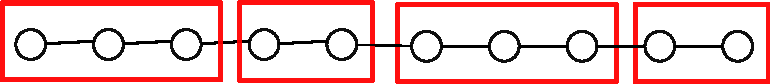
\includegraphics[width=0.9\linewidth]{assets/tmp-code/line_graph.pdf}
  \caption{A line graph with stars in red}
  \label{fig:gtx_line_graph}
\end{marginfigure}
This will results in $\nicefrac{2n}{5}$ stars, which is less than half of $n$ and because in that
case $n=m+1$, \gtx{} will finish after $O(\log m)$ iterations. Note that a barbell graph (two
cliques connected by a line) would requires a number of iterations proportional to the length of that
central line, despite having many more edges. This suggests unsurprisingly that the diameter of the graph
could be a good parameter to quantify the number of iterations needed. Indeed, take a tree and consider
the length $p$ of its longest path from the root to a leaf. By a similar argument as the one used in
the line case, it seems \gtx{} will terminate after $O(\log p)$ iterations.

While all $G_t$ are connected, it might happen during the execution of \extractStar{} that%
\begin{marginfigure}
  \centering
  \includegraphics[width=0.95\linewidth]{assets/tikz/gtx_singleton_tikz.pdf}
  \caption{The formation of a singleton star}
  \label{fig:gtx_singleton}
\end{marginfigure}
the degree of a node $u$ drops to zero because all of its neighbors were claimed by the
periphery of previous stars. Such a node then forms a \emph{singleton star}, as illustrated in
\autoref{fig:gtx_singleton}, where after the creation of \starone{1} and \starone{2}, $c_3$ is the
single node of the third star \starone{3}.%
\begin{marginfigure}
  \centering
  \includegraphics[width=0.95\linewidth]{assets/tikz/gtx_noreduc_tikz.pdf}
  \caption{A case were too many singletons \enquote{waste} one iteration of \gtx{}}
  \label{fig:gtx_noreduc}
\end{marginfigure}
In the case no singleton are formed during one execution of \extractStar{}, the number of nodes is
reduced by at least a factor $2$ (because each star is made of at least two nodes). On the other hand, we can
construct a graph with singletons where the factor of reduction in number of nodes and edges can be
arbitrarily close to $1$. Consider \autoref{fig:gtx_noreduc}, where $c_1$ and $c_2$ have a degree
$p$ and their neighbors (in light gray) all have a degree $q$, which we can vary from $1$ to $p-1$.
At this step $t$, we thus have $|V_t| = 2(1+p)+pq$ and $|E_t| = 2(p+qp)$. Next we run \extractStar{}
and assume that we first extract the two stars centered in $c_1$ and $c_2$. This reduces the
effective degree of all the middle nodes (in dark gray) to $0$ and they thus form singletons, that
are all connected to the first two stars by \collapseStar{}. As a result, at step $t+1$ we have
$|V_{t+1}| = 2 + pq$ and $|E_{t+1}| = 2pq$, so that
\begin{equation*}
\frac{|V_{t+1}|}{|V_t|} = \frac{pq+2}{p(q+2) + 2} \qquad \text{and} \qquad
\frac{|E_{t+1}|}{|E_t|} = \frac{2pq}{2p(q+1)} = \frac{q}{q+1}
\end{equation*}
When we let $p$ goes to infinity, setting $q=1$ makes $\frac{|V_{t+1}|}{|V_t|}$ tend to
$\nicefrac{1}{3}$ and $\frac{|E_{t+1}|}{|E_t|}$ to $\nicefrac{1}{2}$ while setting $q=p-1$ makes
both $\frac{|V_{t+1}|}{|V_t|}$ and $\frac{|E_{t+1}|}{|E_t|}$ tend to $1$. Note however that in both
cases, this is not really a problem because at the next iteration, there will be only two stars (one
of them will be a singleton). Is it always like that? In other words, can we have a situation where
a large number of singletons is carried over several consecutive iterations?

\paragraph{Variants of \extractStar{}}
\label{ssec:gtx_center_choice}

The execution of \extractStar{} is mainly deterministic, except for the fact the ties between nodes
with the same highest degree are broken arbitrarily. While this allows for an efficient
implementation, and simplify the analysis of the resulting sequence of stars and therefore the
induced spanning tree, in can be detrimental in an adversarial context, where we could end up with a
tree forcing a lot of mistakes. We add an element of randomization to \extractStar{} by letting it
use of two optional arguments, a \emph{threshold function} $\tau$ or a \emph{degree function}
$\widetilde{d}$. Such functions modify the center sampling process in the following way:
\begin{itemize}%[nosep]
  \item if $n_{t,i}$ is the number of node remaining in $V_t$ before choosing the \ith{} center, choose
    a node \uar{} among those with a degree larger than $\tau(n_{t,i})$. The idea is to choose
    among a small set of high degree nodes, for instance by letting $\tau(n) = \sqrt{n}$. Note
    however we cannot guarantee there will always be nodes with degree above the threshold, in which
    case we default on the highest degree node
  \item if $\degr_i(u)$ is the degree of node $u$ before choosing the \ith{} center, choose node
    proportionally to $\widetilde{d}(\degr_i(u))$. Again, the degree function is designed so that it
    favors the selection of high degree nodes. For instance, one could use
    $\widetilde{d}(\degr_i(u)) = \degr_i(u)^2$.
\end{itemize}

These two variants are more time consuming because they require additional bookkeeping.
Therefore, we don't provide a full complexity analysis and only briefly sketch their implementations
here.\footnote{Although they are available online at
\nolinkurl{https://github.com/daureg/magnet/blob/master/veverica/}%
\{\href{https://github.com/daureg/magnet/blob/master/veverica/ThresholdSampler.py}%
{ThresholdSampler.py}, \href{https://github.com/daureg/magnet/blob/master/veverica/NodeSampler.py}%
{NodeSampler.py}\}.} For the threshold function, we
maintain two queues, $high$ and $low$, containing nodes whose degree is respectively above and below
the current threshold. We select a node \uar{} in $high$, remove the corresponding star from $G_t$,
recompute the new threshold and if necessary, move nodes which fell under the threshold from $high$
to $low$ and those who climb above the threshold from $low$ to $high$. For the degree function, we
can draw any node as center proportionally to its weight (where the weight of node $u$ is defined as
$d_f\left(\degr(u)\right)$). Yet we cannot use the standard method of computing the cumulative sum
of weights since some of them change at each iteration. Therefore, we construct a binary tree whose
leaves are the nodes of $V_t$ and where each tree nodes maintain the sum of weights in its left and
right subtrees. To sample, we draw a random number $r$ between $0$ and the total weight of the tree and
go down from the root to the leaf spanning the weight interval containing $r$.
When degrees are updated (or graph node removed), we update the weights along a path from the
corresponding leaves to the root of the tree.

A variant of the \gtx{} algorithm as a whole we did not explore so much in practice is its ability
to produce spanner by stopping early. Basically if we stop at iteration $t$, we output the graph
$G_t$ (which in general is not a tree) with its edges unfolded to lie in $E_0$. This corresponds to
a trade off between having more edges than $|V_0|-1$ but potentially making shorter connection and
thus having a lower stretch.


\subsection{Related works}
\label{sub:gtx_related_works}

\label{sub:gtx_state_of_the_art}

Looking for a subgraph $H$ of $G$ that best preserves the distance in $G$ while being sparse is an old
problem, driven originally by network design in fields such as transportation~\autocite{RoadNetworks60}
and electrical circuits~\autocite{electricalNetworks60}. The way we define \enquote{preserving the
distance}, and the exact form of $H$ give rise to several problems, which we summarize later in
\autoref{tab:gtx_related_stretch}. We first give some
definitions, then cover the most relevant problems in details, and finally give some pointers for
the others problems.

Let the distance between $u$ and $v$ in $G$ be
\begin{equation*}
  d_G(u,v) = \sum_{e \in \pathguv} \ell(e)\,,
\end{equation*}
where $\ell(e)$ is the \emph{length} of the edge $e$ and \pathguv{} is the shortest path between $u$
and $v$ in $G$. In the following, we consider only the uniform case, in which the length of an edge
is equal to its weight. The stretch of an edge $(u,v)$ in $H$ is defined as
\begin{equation*}
  \estr(u,v) = \frac{d_H(u,v)}{d_G(u,v)}.
\end{equation*}

We may then want to minimize the stretch of:
\begin{enumerate}[1),nosep]%,leftmargin=*]
  \item some pairs of nodes. That is, given $L$ and $R$ in $V$, minimize $\sum_{u \in L, v\in R}
    \estr(u,v)$
  \item all pairs of nodes corresponding to edges of $G$, \ie{} minimize $\sum_{(u,v) \in E}
    \estr(u,v)$
  \item all pairs of nodes, \ie{}  minimize $\sum_{(u,v) \in V^2} \estr(u,v)$
\end{enumerate}
Note that for unweighted graphs, the second problem reduces to minimizing
\begin{equation}
  \label{eq:test_stretch_def}
  \estr(H) = \sum_{(u,v) \in E} |\pathhuv|.
\end{equation}
If furthermore $H$ is tree, this is equivalent to minimize the second term of equation
\eqref{eq:stretch_mistakes}. Therefore we focus mainly of that definition of stretch, and consider
the other two only briefly.

The second point affecting the problem is the structure of $H$. The only requirements are that it
must be spanning all the nodes involved in the computation of the chosen stretch, and that $\forall
(u,v) \in E,\, d_H(u,v) \geq d_G(u,v)$. Beside that, $H$ can be a tree of $G$, a general subgraph of
$G$ or even a subset of $V^2$ (\ie{} containing edges not in $E$). We focus mainly on the first two
cases, since they are covered by the \gtx{} algorithm.

% Namely, let $G$ be a graph over vertex set $V$ with $|V|=n$ and edge set $E$. Furthermore, let $T$
% be a spanning tree of $G$ and $\etest{}$ the edges of $G$ not in $T$. Then we define the
% \emph{average test edge stretch} as $\frac{1}{|\etest{}|} \sum_{(u,v) \in \etest{}}
% |\mathrm{path}^T_{u,v}|$, where $|\mathrm{path}^T_{u,v}|$ is the unique path between $u$ and $v$ in
% $T$.


% However, \textcite[Section 3, page 453]{lognMetricBoundConf03} claim a $O(\log n)$ approximation so maybe I'm
% wrong. Turns out, they refer to a distribution over trees and this $O(\log n)$ is the expected
% stretch of a tree sampled from this distribution

% This defines two kind of structures, spanning trees and spanners (which are still sparse subgraphs
% yet containing more than $|V|-1$ edges).

\paragraph{Trees}
\label{par:trees}

One early mention of seeking a low-stretch spanning tree is given by \textcite{Requirements74},
albeit in more general form:
\begin{problem}[Optimal Communication Spanning Tree]
Given a set of nodes $V=\{v_1, \ldots, v_n\}$, a set of distances $d_{ij}$ and a set of requirements
$r_{ij}$ between $v_i$ and $v_j$, find a spanning tree connecting these $n$ nodes such that the
total cost of communication of the spanning tree is a minimum among all spanning trees. The cost of
communication for a pair of nodes is $r_{i,j}$ multiplied by the sum of the distances of arcs which
form the unique path connecting $v_i$ and $v_j$ in the spanning tree. The cost of a spanning tree is
the sum of costs over all pairs of nodes.
\end{problem}
For a weighted graph $G=(V,E,w)$, by letting $d_{ij} = w_{ij}$ and $r_{i,j}= \Ind{(i,j) \in E}$,
finding an Optimal Communication Spanning Tree thus amounts to finding a low-stretch spanning tree.
\autoref{tab:gtx_related} present a list of works where the stretch was improved.

We start with the seminal paper of \textcite{LowerBound95}. It touches on many topics, and frame the
problem in a game theoretic way but here we only focus on two of their results: a lower bound of
$\Omega(\log n)$ for the average stretch of any tree and their construction of a tree with $\exp
O(\sqrt{\log n\log\log n})$ average stretch in time $O(m^2)$. The lower bound follows from an
existing result in extremal graph theory~\autocite[pages 107--109]{ExtremalGraph04}: there is a
positive constant $a$ such that for all $n\in \Nbb$, one can construct a graph $G$ with $n$ vertices
and $2n$ edges such that every cycle $G$ has a length of at least $a\log n$. Now consider any
spanning tree $T$ of $G$.  While all the $n-1$ edges of $T$ have a stretch of $1$, the $n+1$
remaining ones form a cycle in $T$ hence in $G$ as well and thus incur a stretch of at least $a\log
n$. This shows that the average stretch is at least $\frac{1}{2}a\log n$.

They construct a low stretch spanning tree in a bottom up manner like the \gtx{} algorithm. First,
they extend the definition of stretch to multigraph~\autocite[Section 4]{LowerBound95} and then
describe a procedure to transform in linear time any multigraph $G$ with $n$ nodes to a multigraph
$G'$ on the same nodeset with at most $n(n+1)$ edges such the average stretch of $G'$ is at most
twice that of $G$~\autocite[Lemma 5.2]{LowerBound95}. The next ingredient is an algorithm to build a
low diameter decomposition of a multigraph $G$, parametrized by a number $x(n)$ depending of $n$. It
works by repeatedly selecting an arbitrary node and growing a ball around it until the number of
edges leaving the ball is at most a fraction $\nicefrac{1}{x(n)}$ of the number of edges with both
endpoints in the ball. The key property of this decomposition is that it yields a partition of $G$
in clusters such that the radius of each cluster is small (namely at most $O(x(n)\log n)$) and there
is most a fraction $\nicefrac{1}{x(n)}$ of edges between clusters. Finally, the iterative procedure
is a follows: once a partition has been built, we compute a shortest path spanning tree in each
cluster that are then collapsed into super nodes to form the next graph $G'$ and the process repeats.
Another difference from \gtx{}, besides the partition procedure, is that $G'$ is a multigraph,
taking into account the number of edges joining cluster, while \collapseStar{} picks only the most
direct one.

Another interesting idea from this paper is to consider a distribution over trees instead of a
single instance, especially when one is concerned about the maximum stretch instead of the average
one. For instance, on a cycle with $n$ nodes, a tree is obtained by removing one edge, and that edge
incurs a stretch of $n-1$. The uniform distribution over such trees has a maximum stretch of
$2\left(1 - \frac{1}{n}\right)$~\autocite{circle2k89}.

\begin{table}[htbp]
  \centering
  \caption{Reproduction of Table 1 from~\autocite{Abraham2012}, showing the evolution of the best
  asymptotic average stretch over time.}\label{tab:gtx_related}
  \begin{tabular}{lll}
    \toprule
    work                      & average stretch                          & time                    \\
    \midrule
    \autocite{LowerBound95}   & $\exp(O(\sqrt{\log n\log\log n}))$       & $O(m^2)$                \\
    \autocite{LowerStretch05} & $O((\log n)^2 \log \log n)$              & $O(m \log^2 n)$         \\
    \autocite{nearlyTight08}  & $O(\log n(\log \log n)^3)$              & $O(m \log^2 n)$         \\
    % \autocite{nearlyTight08}  & $O(\log n \log\log n(\log\log\log n)^3)$ & $O(m^2)$                \\
    \autocite{TighterSDD11}   & $O(\log n(\log \log n)^3 )$              & $O(m \log n\log\log n)$ \\
    \autocite{Abraham2012}    & $O(\log n \log \log n)$                  & $O(m \log n\log\log n)$ \\
    \bottomrule
  \end{tabular}
\end{table}

The idea of recursively partitioning the graph and construction a low-stretch spanning tree in each
part is common to all the papers of \autoref{tab:gtx_related}. \Textcite{LowerStretch05} devise a
$(\delta, \epsilon)$-star decomposition such that all the stars have comparably low radius.
It was modified in~\autocite{nearlyTight08} to improve the stretch. Then \textcite{TighterSDD11}
improve the runtime by rounding the edge weights to the closest power of $2$ and using a modified
implementation of the Dijkstra's algorithm in the case of at most $k$ distinct edge
weights~\autocite{FastPathFewWeights10}. Finally, \textcite{Abraham2012} describe an even more
complex but tighter petal decomposition.
\iffalse
\begin{marginfigure}
  \centering
  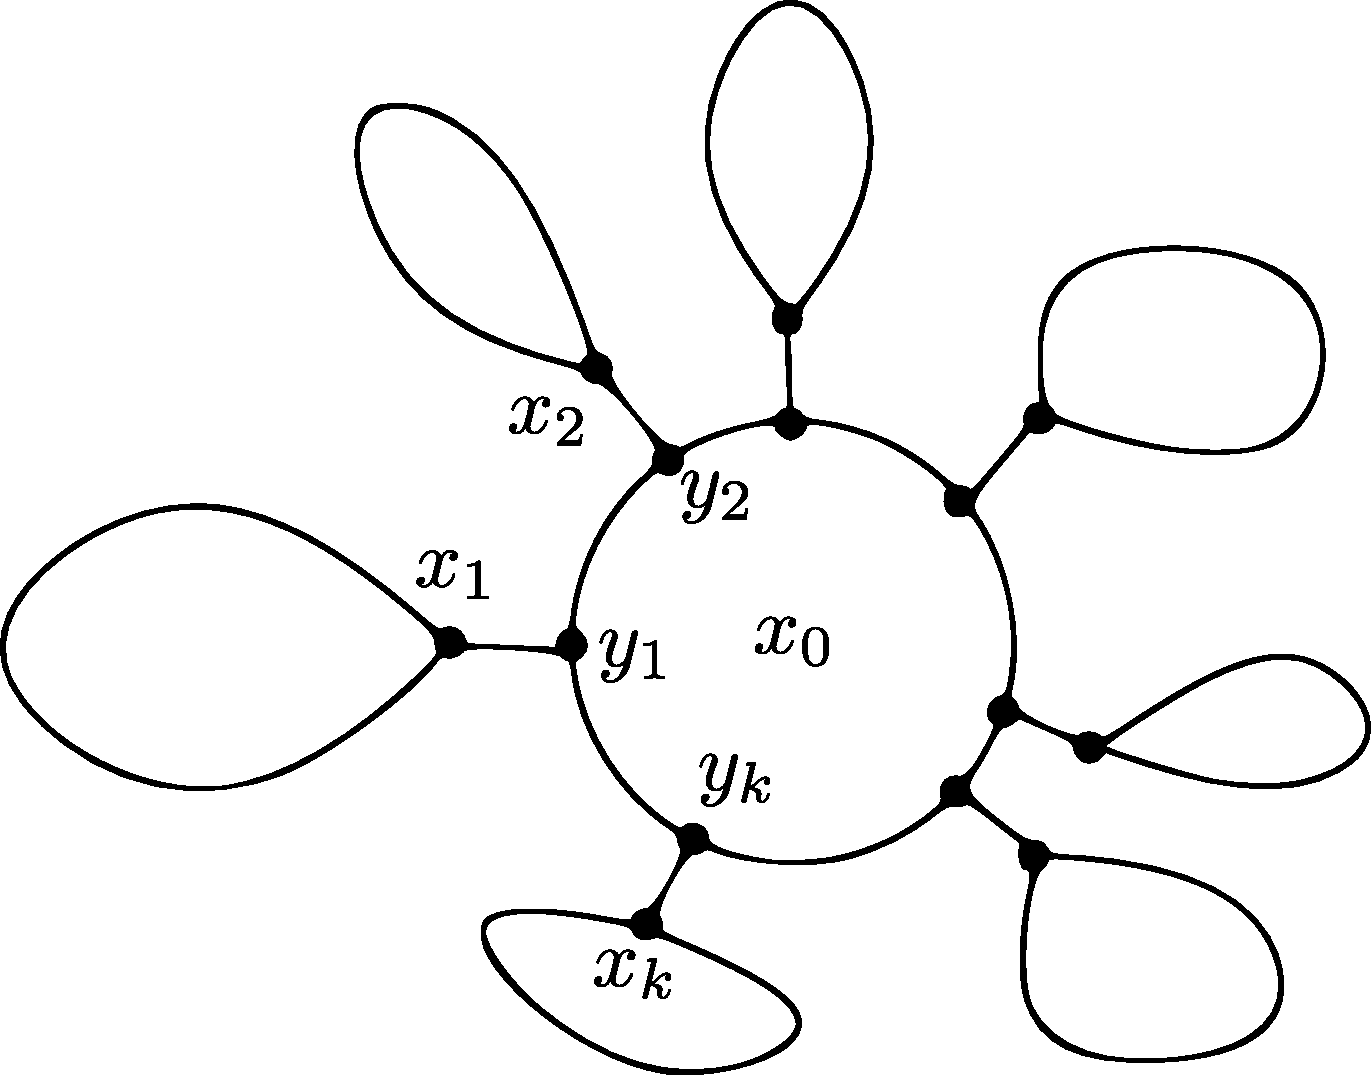
\includegraphics[width=.95\textwidth]{assets/raw/star_decomp.pdf}
  \caption{Star decomposition (reproduced from Figure 1 of~\autocite{LowerStretch05})}
  \label{fig:gtx_star_decomp}
\end{marginfigure}

Special case of graph
series parallel
\enquote{In a subsequent paper, \textcite{seriesParallel06} proved that every series-parallel
unweighted graph admits a spanning tree of average stretch $O(log n)$. This bound is tight as it
matches the lower bound established in~\autocite{cutsTrees99}.}

more special cases are in~\autocite{specialCase14}, although it's for the minimum max stretch
$t^\star$.
\enquote{Note also that a number of particular graph classes (like interval
graphs, permutation graphs, asteroidal-triple–free graphs, strongly chordal graphs,
dually chordal graphs, and others) admit tree $t$-spanners for small values of $t$}
\fi


\paragraph{Spanners}
\label{par:spanners}

As we mentioned, by stopping the \gtx{} algorithm before it finishes, we obtain a set of edges
spanning the graphs that is not a tree. Such structure are called \emph{spanner}. More precisely,
the subgraph $H$ is said to be an $t$-spanner of $G$ if, for a parameter $t \geq 1$, and for every
pair $u, v \in V$ of vertices, it holds that $d_H(u, v) \leq t \cdot d_G(u, v)$. The problem was
introduced by \textcites{SpannerFirst89}{SpannerSecond89} and has been extensively studied since
then, for it has many applications in network design. It was also showed to be \NPh{} to
approximate~\autocite{SpannerNPHard07}. The most simple construction is a greedy
algorithm~\autocite{greedySpanner93} that works similarly to the minimum spanning tree construction.
Starting from an empty subgraph $H$, it goes through every edge $(u, v)$ of $G$ sorted by weight and
check if there is a path between $u$ and $v$ in $H$ of length at most $t$. If this is the case, the edge
$(u,v)$ is dropped, otherwise it is inserted in $H$. This results in a $(2t - 1)$-spanner with
$O(n^{1+1/t})$ edges, which is an optimal trade-off between those two quantifies.  Furthermore on
weighted graphs, the greedy spanner total weight is essentially optimal~\autocite{GreedyOpt16}.
However, the best implementation of it, using a dynamic data structure~\autocite{fastGreedy04} is
not scalable for it runs in $O(t n^{2+\nicefrac{1}{t}})$ and cannot easily be parallelized.
Parallelization therefore requires other kind of approaches~\autocites{parSpanner08}{parSpanner15}.
Recently, \textcite{Spanner17} showed how to obtain, for any $\epsilon > 0$, a $(2t - 1)$-spanner
with $O(n^{1+1/k}/\epsilon)$ edges in $t$ rounds, with probability at least $1 - \epsilon$.

\iffalse
\url{http://www.siam.org/meetings/da17/schedule.html} SODA 13B \url{http://dl.acm.org/citation.cfm?id=3039686}
for instance the Elkin paper~\autocite{Spanner17} \enquote{Our centralized randomized algorithm computes (with
probability close to 1), a $(2k - 1)$-spanner with $n \cdot (1 + O(\frac{\log k}{n}))$ edges in
$O(|E|)$ time, whenever $k = \Omega(\log n)$. Note that when $k = \omega(\log n)$, the number of
edges is $n(1+o(1))$, i.e., in this range the algorithm computes an ultra-sparse spanner in $O(|E|)$
time.} For instance, if $k=5\log n$, we get a $10\log n$-spanner with $n\left(1+O\left(\frac{\log\log
n}{n}\right)\right)$ edges in $O(|E|)$ time.


They have applications in computing approximately shortest
paths [9, 22, 28, 37], routing [48], distance oracles and
labeling schemes [49, 56, 36] and synchronization [7].

From 6:They also appear in biology in the process of reconstructing phylogenetic trees from
matrices, whose entries represent genetic distances among contemporary living species (H. J.
Bandelt, A. W. M. Dress, Reconstructing the Shape of a Tree from Observed Dissimilarity Data, Adv.
in Appl. Math. 7 (1986)). Robotics researchers have studied spanners under the constraints of
Euclidean geometry, where vertices of the graph are points in space, and edges are line segments
joining pairs of points (Chew), (Dobkin), $[DJ], [K], [KG], [LL]$. 

studied in 1; 4; 6; 9; 15; 19; 22; 24; 26; 28; 30; 31; 37; 43; 51; 52; 57; 58



\begin{tabulary}{\textwidth}{LLLLL}
  \toprule
  work  & average stretch & edge size                              & weighted & time                                             \\
  \midrule
  46    & $4k + 1$        & $O(n^{1+\nicefrac{1}{k}})$             & no       & polynomial                                       \\
  6     & $2k +1$         & $O(n\cdot \ceil{n^{\nicefrac{1}{k}}})$ & yes      & $O\left(m(n^{1+\nicefrac{1}{k}}+n\log n)\right)$ \\
  40    & $2k-1$          & $O(n^{1+\nicefrac{1}{k}}+n)$           & no       & $O(m)$                                           \\
  Elkin & $2k-1$          & $n \cdot (1 + O(\frac{\log k}{n}))$    & no       & $O(m)$                                           \\
  \bottomrule
\end{tabulary}

% 22: E. Cohen, "Fast algorithms for constructing t-spanners and paths with stretch t," Proceedings
% of 1993 IEEE 34th Annual Foundations of Computer Science, Palo Alto, CA, 1993, pp. 648-658.  doi:
% 10.1109/SFCS.1993.366822
% We construct t-spanners of size (number of edges) Õ(n 1+(2+\epsilon)/t )
% (for any \epsilon > 0 and t such that t/(2+\epsilon) is integral). These spanners can be constructed
% by a randomized algorithm that runs in Õ(mn (2+\epsilon)/t ) time.


% Halperin and Zwick [40].  Their deterministic algorithm, for an integer parame- ter k ≥ 1,
% computes a (2k − 1)-spanner with n 1+1/k + n edges in O(|E|) time. (Their result improved previous
% pioneering work by [46, 22].)

Describe the greedy algorithm of 6. Using (55 On Dynamic Shortest Paths Problems Liam Roditty, Uri
Zwick, 2004), it runs in $O(\alpha n^{2+\nicefrac{1}{\alpha}})$

peleg 2007 hardness results

46: Peleg, D. and Schäffer, A. A. (1989), Graph spanners. J. Graph Theory, 13: 99–116.
doi:10.1002/jgt.3190130114

study the problem on unweighted graph. Application to routing scheme (48: D. Peleg and E. Upfal, A
tradeoff between space and efficiency for routing tables. 20th ACM Symposium on the Theory of
Computing, Chicago (1988))
Special case for the complete graph weighted by the distance in a 2D plan. Existing $\sqrt{10}$
spanner for the $\ell_1$ metric (L. P. Chew, There is a planar graph almost as good as the complete
graph.  Proceedings of the 2nd ACM Symposium on Computational Geometry, (1986)) (improved to
$\sqrt{4+2\sqrt{2}}$ by N. Bonichon, C. Gavoille, N. Hanusse, L. Perkovic The stretch factor of
$\ell_1$ and $\ell_{\infty}$ Delaunay triangulations European Symposium on Algorithms (ESA) (2012))
and $\phi \pi$ for $\ell_2$ (D. P. Dobkin, S. J. Friedman, and K. J. Supowit, Delaunay graphs are
almost as good as complete graphs. 28th IEEE Symposium on the Foundations of Computer Science,
(1987)) (improved to $1.998$ by Ge Xia. 2011. Improved upper bound on the stretch factor of delaunay
triangulations. In Proceedings of the twenty-seventh annual symposium on Computational geometry
(SoCG '11)). See (Prosenjit Bose, Michiel Smid, On plane geometric spanners: A survey and open
problems, Computational Geometry, Volume 46, Issue 7, 2013) for more on the 2D case.

In undirected graph, finding a spanner with less than $k$ edges is \NPc{} (theorem 2.2)
For $k<n$, one can construct in polynomial time a $(4\log_k n +1)$ spanner with less than $kn$ edges
(theorem 2.4) giving for instance ($k=2$) $O(\log n)$ spanner with $O(n)$ edges and
($k=n^{\nicefrac{1}{r}}$, $r\geq 1$) a $(4r+1)$ spanner with $O(n^{1+\nicefrac{1}{r}})$ edges
(matching lower bound within constant factor). For every $d \geq 0$, the $d$-dimensional cube has a
$3$-spanner with fewer than $7\time 2^d$ edges (Lemma 2.10 from 47: D. Peleg and J. D. Ullman. An
optimal synchronizer for the hypercube. SIAM J. on Comput., 18:740–747, 1989)
For chordal graphs: for every $n$-vertex chordal graph there exists a $2$-spanner with
$O(n\sqrt{n})$ edges (matching lower bound), a $3$-spanner with $O(n \log n)$ edges and a $5$-spanner
with $O(n)$ edges.
Much more difficult for directed graph, according to Theorem 4.2: For every $t \geq 1$ there are
infinitely many $n$-vertex directed graphs for which every $t$-spanner requires
$\Omega(\nicefrac{n^2}{t^2})$ edges.

% check some surveys of the 80's
% http://pubsonline.informs.org/doi/abs/10.1287/trsc.18.1.1
% http://onlinelibrary.wiley.com/doi/10.1002/net.3230190305/full
% early solutions
% http://onlinelibrary.wiley.com/doi/10.1002/net.3230090104/full
% http://onlinelibrary.wiley.com/doi/10.1002/net.3230130309/full
% later solution?
% http://ieeexplore.ieee.org/document/81738


While they have many applications [see first paragraph of \url{https://arxiv.org/pdf/1401.2454.pdf},
which was later merged in a STOC'14 paper] (a major one being solving linear systems), in some
practical situations their advantages are less clear [from
\url{https://link.springer.com/chapter/10.1007/978-3-319-20086-6_16}\enquote{for reasonable inputs
the constant factors make the solver much slower than methods with higher asymptotic complexity.
One other aspect predicted by theory is confirmed by our findings: Spanning trees with lower
stretch indeed reduce the solver's running time. Yet, simple spanning tree algorithms perform
better in practice than those with a guaranteed low stretch.} this is improved by
\url{https://link.springer.com/chapter/10.1007%2F978-3-319-20086-6_17} although they seem to work
	mostly with the Laplacian of the tree ]
\fi

\paragraph{Other problems}

Finding low stretch trees and spanners with respect to the existing edges is the most relevant
problem when addressing the \esp{} problem. For the sake of completeness, we nonetheless give an
overview of some related problems.

For instance, \textcite{Johnson1978} define the following problem, where the stretch is defined over
all possible pairs of nodes\footnote{We adapt their notations
to match ours}:  
\begin{problem}[Network Design Problem]
  \label{prob:gtx_ndp}
  Given an undirected integer-weighted graph $G=(V, E, w)$, a budget $B\in\Nbb$ and a criterion
  threshold $C\in \Nbb$, does there exist a spanning subgraph $G'=(V, E')$ of $G$ with weight
  $w(E') \leq B$ and criterion value $F(G') \leq C$, where the criterion function $F(G')$ denotes
  the sum of the weights of the shortest paths in $G'$ between all vertex pairs?
\end{problem}
They prove that finding such a subgraph is \NPc{}, by exhibiting a reduction from the
\textsc{Knapsack} problem. They also prove that the less general problem of finding a spanning tree
on an unweighted graph, that is
\vspace{-.5\baselineskip}
\begin{problem}[Simple Network Design Problem]
  \autoref{prob:gtx_ndp} with $w$ being the equal to $1$ for all edges in $E$ and $B=|V|-1$.
\end{problem}%
\vspace{-.5\baselineskip}
\noindent is also \NPc{} by reduction from \textsc{Exact 3-Cover}.
However, it has recently been show that this Simple Network Design problem can be approximated to a
constant factor $6$~\autocite{AllPairStrech10}. Moreover, even when the graph is weighted,
\textcite{constantDistortion07} achieve a universal constant bound for any weighted graph.

Another problem appear when the low-stretch structure $H$ can include edges not in $G$ (as long as
the distances in $H$ remain larger than the distances in $G$). This is captured by the following
problem~\autocite{OptimalNetwork69}:
\begin{problem}[Optimal Network Problem]
  \label{prob:gtx_scott}
  Given a set $V$ of $n$ vertices, find a set of spanning edges $E\subset V^2$ that minimizes
  the sum of the length of the shortest paths  between all vertex pairs while the
  total length of the resulting network does not exceed some upper bound $B\in\Nbb$.
\end{problem}
This can be seen as a special case of \autoref{prob:gtx_ndp} with $G$ being the unweighted
$n$-complete graph. \Textcite{OptimalNetwork69} proposes a backtracking solution and two local search approximate
algorithms. Some early branch and bound heuristic solutions to \autoref{prob:gtx_scott} are surveyed
in~\autocite[Section 2.3.2]{networkDesignSurvey89} although they do not come with asymptotic
guarantee on the stretch. Furthermore, \textcite{optimApproxNP80} proves that for any $\epsilon \in
(0,1)$, finding a $|V|^{1-\epsilon}$ approximation is \NPc{}.
However, if we consider the average stretches over a distribution of trees, then this approximation
factor can be reduced to $\Theta(\log n)$~\autocite{lognMetricBoundConf03}.

Finally, the stretch can also be computed for a subset of the edges. This is useful in cases where
we have prior information on the importance of individual nodes or edges.  For instance,
\textcite{RamseyTree17} show that for every $t$, any $n$-nodes graph $G=(V,E)$ has a subset $S$ of
size at least $n^{1 - \nicefrac{1}{k}}$, and a spanning tree that has stretch $O ( k \log \log n)$
between any node in $S$ and any node in $V$. Likewise, \textcite{mLAST17} describe how to maintain a
light subgraph $H$ that minimizes the distance between pairs of source and sink that are given in an
online fashion.

As shown by \autoref{tab:gtx_related_stretch}, those problems defined in the seventies are still
being discussed nowadays in top tier conferences, proving their relevance and impact beyond the
\esp{} problem.

\setlength{\fullpage}{179mm}
\begin{table}[htbp]
\begin{adjustwidth}{-2cm}{}
  \centering
  \caption{A summary of the lowest stretches achievable for various problems.
  \label{tab:gtx_related_stretch}}
  \begin{tabulary}{\fullpage}{LCCL}
    \toprule
    kind of stretch    & \multicolumn{2}{c}{only existing edges}  & extra edges allowed   \\
    \midrule
                       & tree                                     & not tree             &\\
    \cmidrule(r){2-3}
    some pairs         & $O(k\log\log n)$~\autocite{RamseyTree17} & \autocite[Section 4]{mLAST17} & --- \\
    all existing pairs & $O\left(\log n (\log\log n)\right)$~\autocite{Abraham2012}
		       & $(2t - 1)$-spanner, $O(n^{1+1/t})$ edges~\autocite{greedySpanner93}
		       & $\Theta(\log n)$ in expectation~\autocite{lognMetricBoundConf03} \\
    all possible pairs & $6$ for unweighted graphs \autocite{AllPairStrech10} and $O(1)$
                         in general \autocite{constantDistortion07}
		       & ---
		       & no need for extra edges in that case                              \\
    \bottomrule
  \end{tabulary}
\end{adjustwidth}
\end{table}


\subsection{Empirical evaluation}
\label{sub:gtx_empirical_evaluation}

In this section, we provide empirical evidences of the properties of
\gtx{} over several classes of graph, and compare it with a \bfs{} baseline.
%\marginpars{If time allows, it would be interesting to implement some methods of \vref{sub:gtx_state_of_the_art} and add them to the comparison}\todo*{implement more low stretch methods}
Namely, we consider three kinds of
graph topology (with both synthetic and real world instances that carry signs on their edges) and
evaluate $(i)$ what average stretch is reached by various trees and $(ii)$ how accurate is the sign
prediction.

\subsubsection{Graph topology}

The three kinds of topology we consider are:
\begin{description}[leftmargin=*]
	\item[\grid{}] which are 2D lattices, where each node has four neighbors except on the boundary.
		The synthetic ones are square, while the \enquote{real world} ones represents the four neighbors
		pixel connectivity of the pictures showed in \autoref{fig:gtx_xp_bwpics}.
	\item[\lpa{}] which are built synthetically according to the model of \textcite{Barabasi1999}.
		While this does not follow the more rigorous specification of \textcite{PAmodel04}, informally,
		we start with a line graph of $m$ nodes and add node one by one until the graph consists of $n$
		nodes. Each time a new node is added, it is connected to $m$ of the existing nodes with a
		probability proportional to their degree. Here we choose $m=3.13$, that is when adding a new
		node, we pick $3$ or $4$ existing neighbors such the initial expected number of neighbors for
		each new nodes is $3.13$. Such graphs are quite sparse and have short diameter, thus providing a
		crude but reasonable approximation of online social networks. Therefore, the real world
		instances of the \lpa{} model are \wik{}, \sla{} and \epi{} networks from \autoref{chap:troll}
		 along with \gplus{}. The last one is constructed from
		ego networks of \gplus{}\footnote{Available at
		\url{http://snap.stanford.edu/data/egonets-Gplus.html}} by keeping the largest connected
		component of users whose gender is known. Basic statistics of those real \lpa{} graphs are
		presented in (\autoref{tab:gtx_xp_dataset}). 
	\item[\triangle{}] which consists of a Delaunay triangulation of a set of points randomly
		located in a 2D space.\footnote{As
		implemented by the \textsf{graph-tool} library (\url{https://graph-tool.skewed.de})}
\end{description}

\begin{table}[htpb]
	\centering
	\caption{Dataset description }\label{tab:gtx_xp_dataset}
	\begin{tabular}{lrrcc}
		\toprule
             & $|V|$  & $|E|$    & fraction of $+$ edges & $\frac{2|E|}{|V|\cdot(|V|-1)}$ \\
		\midrule
		\wik{}   & \np{7065}   & \np{99936}    & 78.5\%                & $4.00\cdot 10^{3}$             \\
		\gplus{} & \np{74917}  & \np{10130461} & 67.6\%                & $3.61\cdot 10^{3}$             \\
		\sla{}   & \np{82052}  & \np{498527}   & 76.4\%                & $1.48\cdot 10^{4}$             \\
		\epi{}   & \np{119070} & \np{701569}   & 83.2\%                & $9.90\cdot 10^{5}$             \\
		\bottomrule
	\end{tabular}
\end{table}

\begin{figure}[t]
	\centering
	\begin{subfigure}[b]{0.32\textwidth}
		
\includegraphics[width=\textwidth]{gtx_exp/zmonastery}
	\end{subfigure}~
	\begin{subfigure}[b]{0.32\textwidth}
		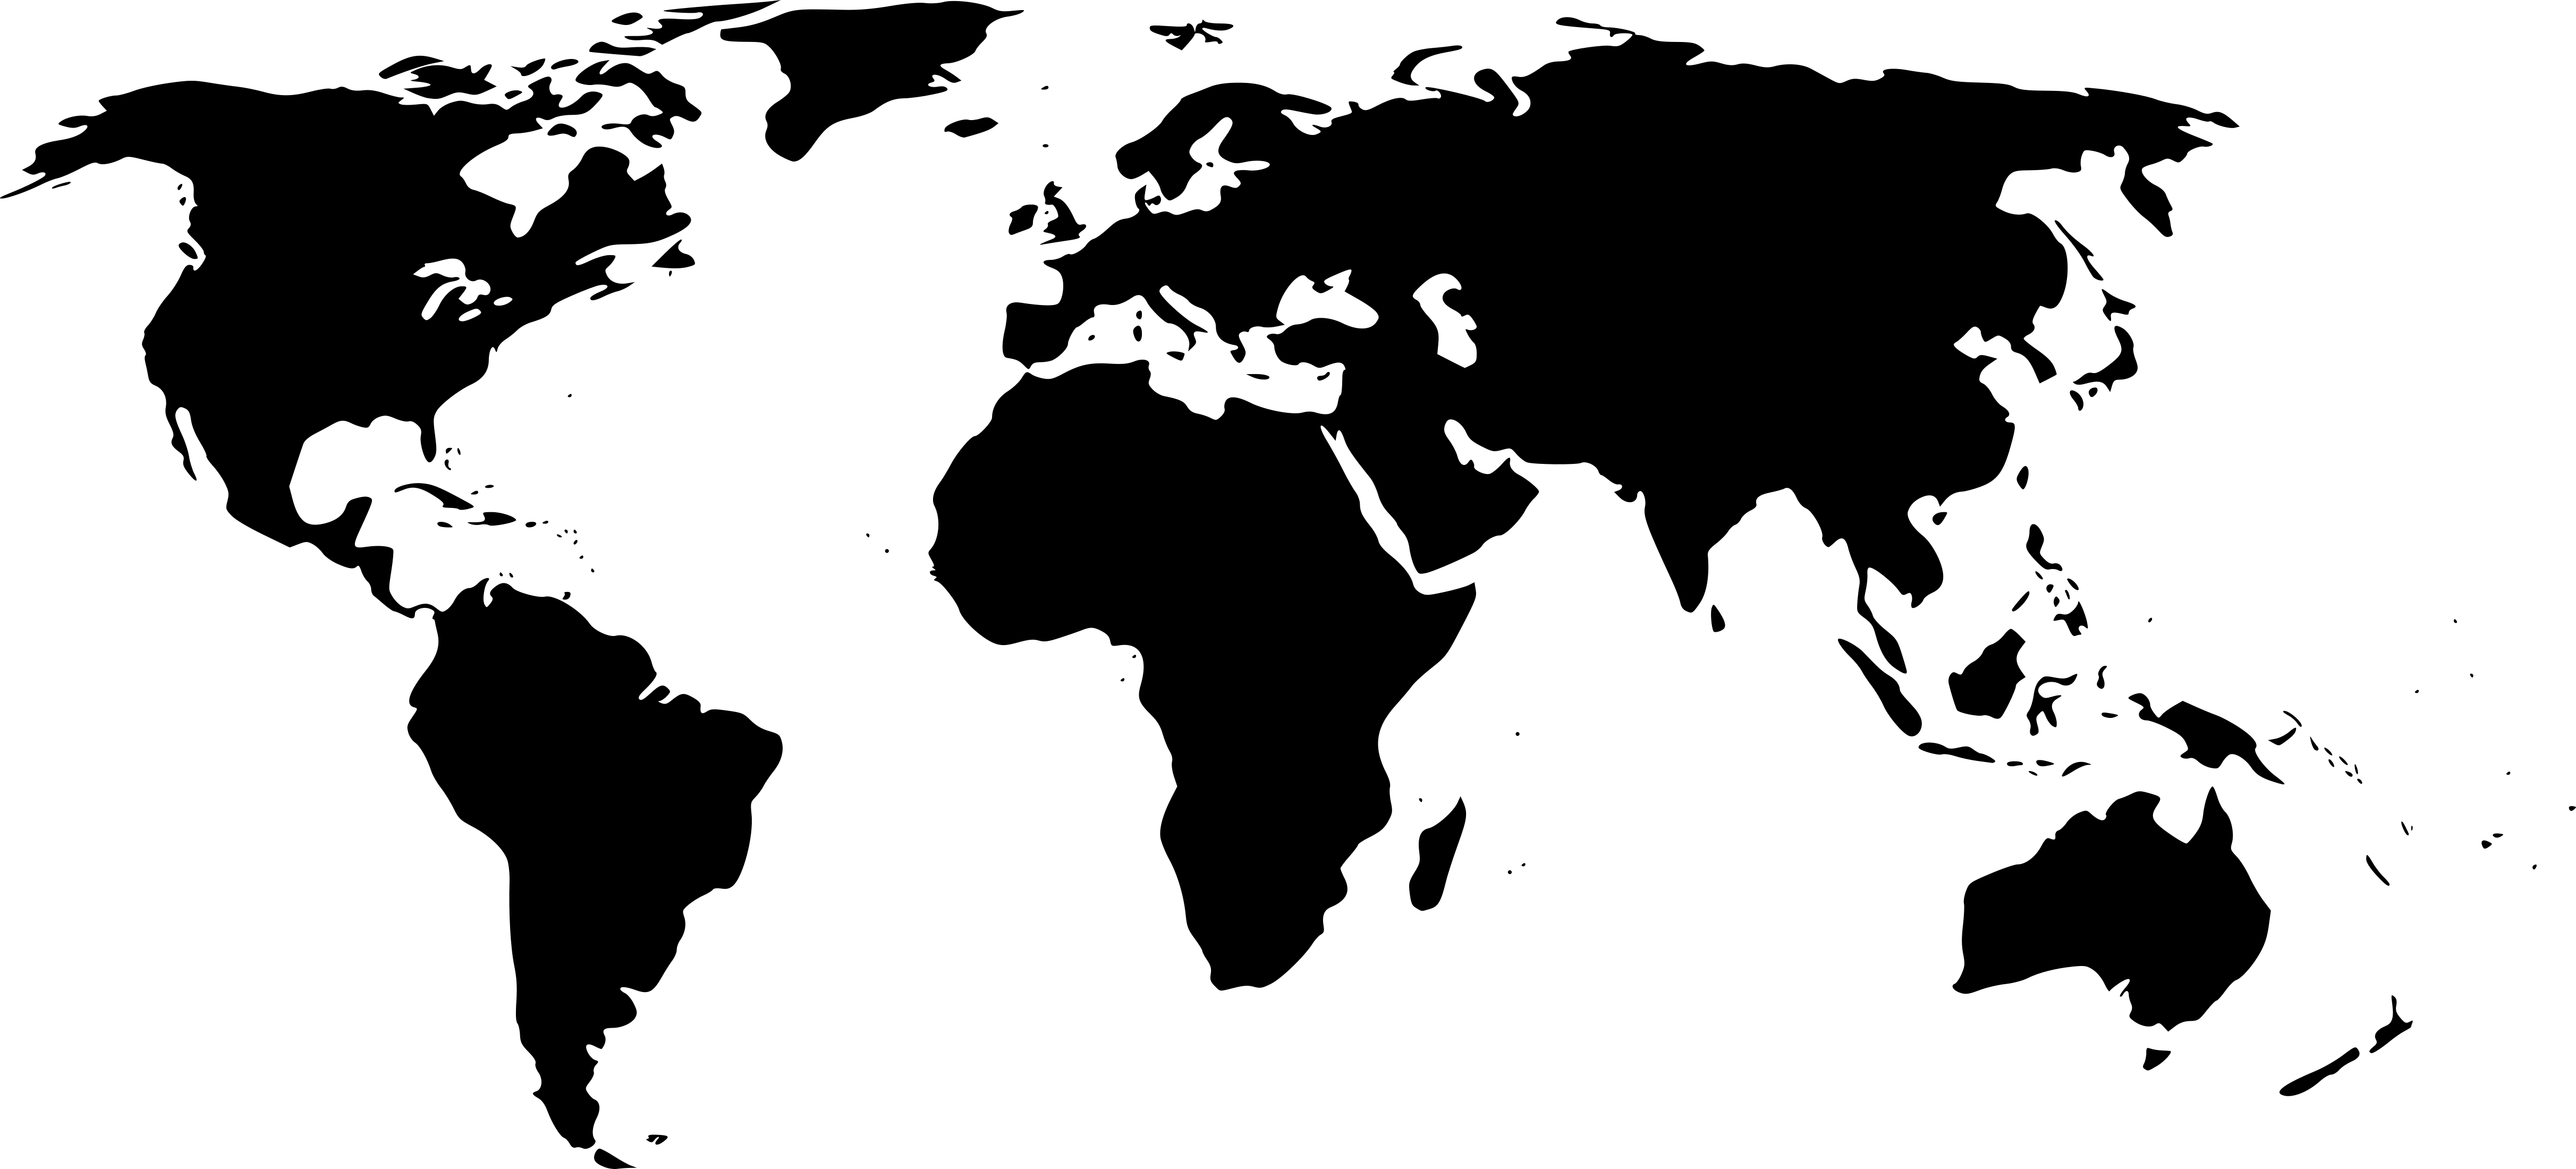
\includegraphics[width=\textwidth]{gtx_exp/zworld}
	\end{subfigure}~
	\begin{subfigure}[b]{0.32\textwidth}
		
\includegraphics[width=\textwidth]{gtx_exp/nips_poster}
	\end{subfigure}

	\begin{subfigure}[b]{0.32\textwidth}
		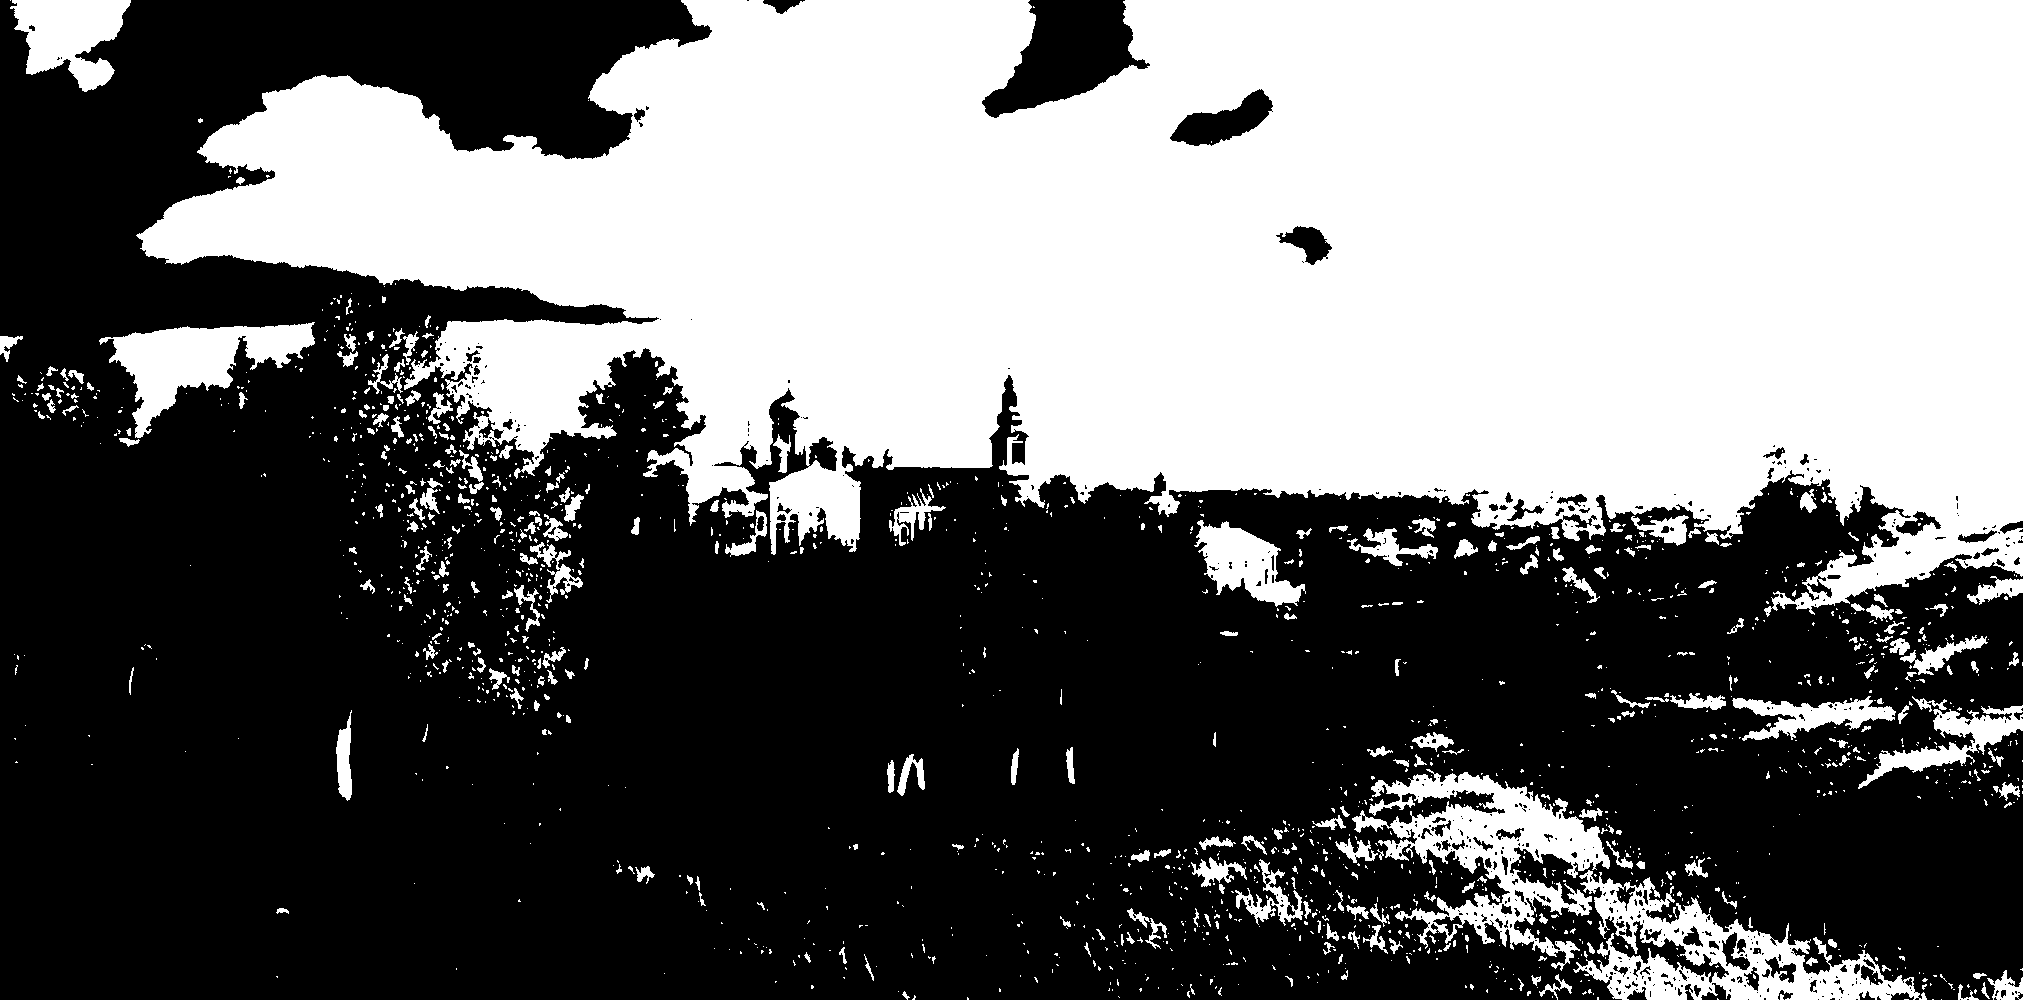
\includegraphics[width=\textwidth]{gtx_exp/zmonastery_bin}
		\caption{monastery}
	\end{subfigure}~
	\begin{subfigure}[b]{0.32\textwidth}
		
\includegraphics[width=\textwidth]{gtx_exp/zworld_bin}
		\caption{world}
	\end{subfigure}~
	\begin{subfigure}[b]{0.32\textwidth}
		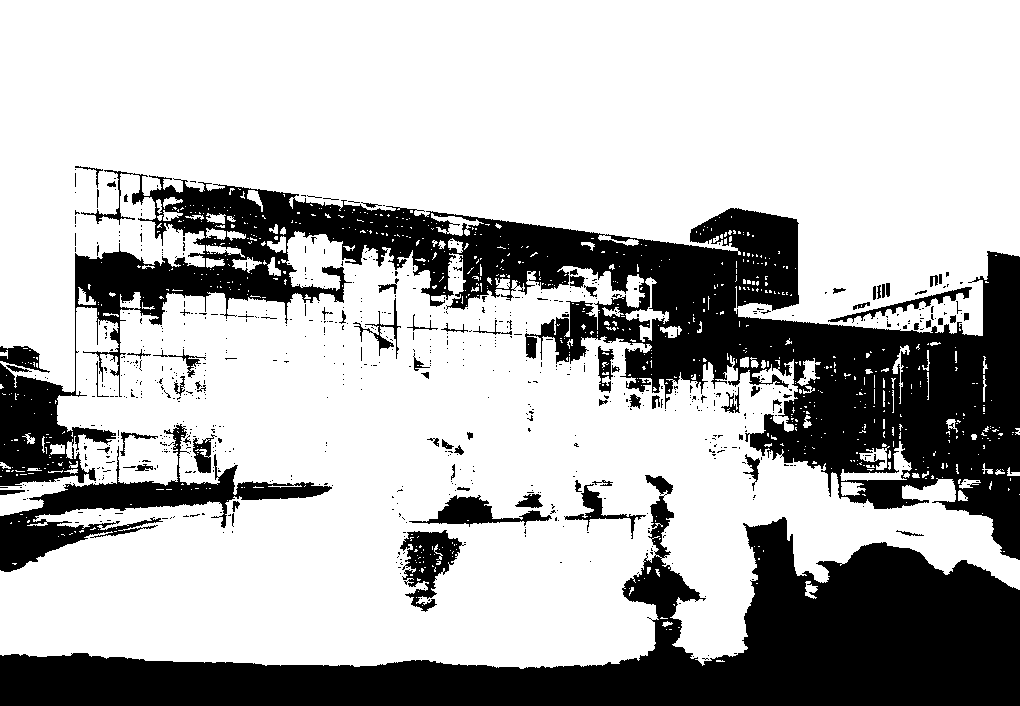
\includegraphics[width=\textwidth]{gtx_exp/nips_poster_bin}
		\caption{poster}
	\end{subfigure}

	\begin{subfigure}[b]{0.32\textwidth}
		
\includegraphics[width=\textwidth]{gtx_exp/nips_logo}
	\end{subfigure}~
	\begin{subfigure}[b]{0.32\textwidth}
		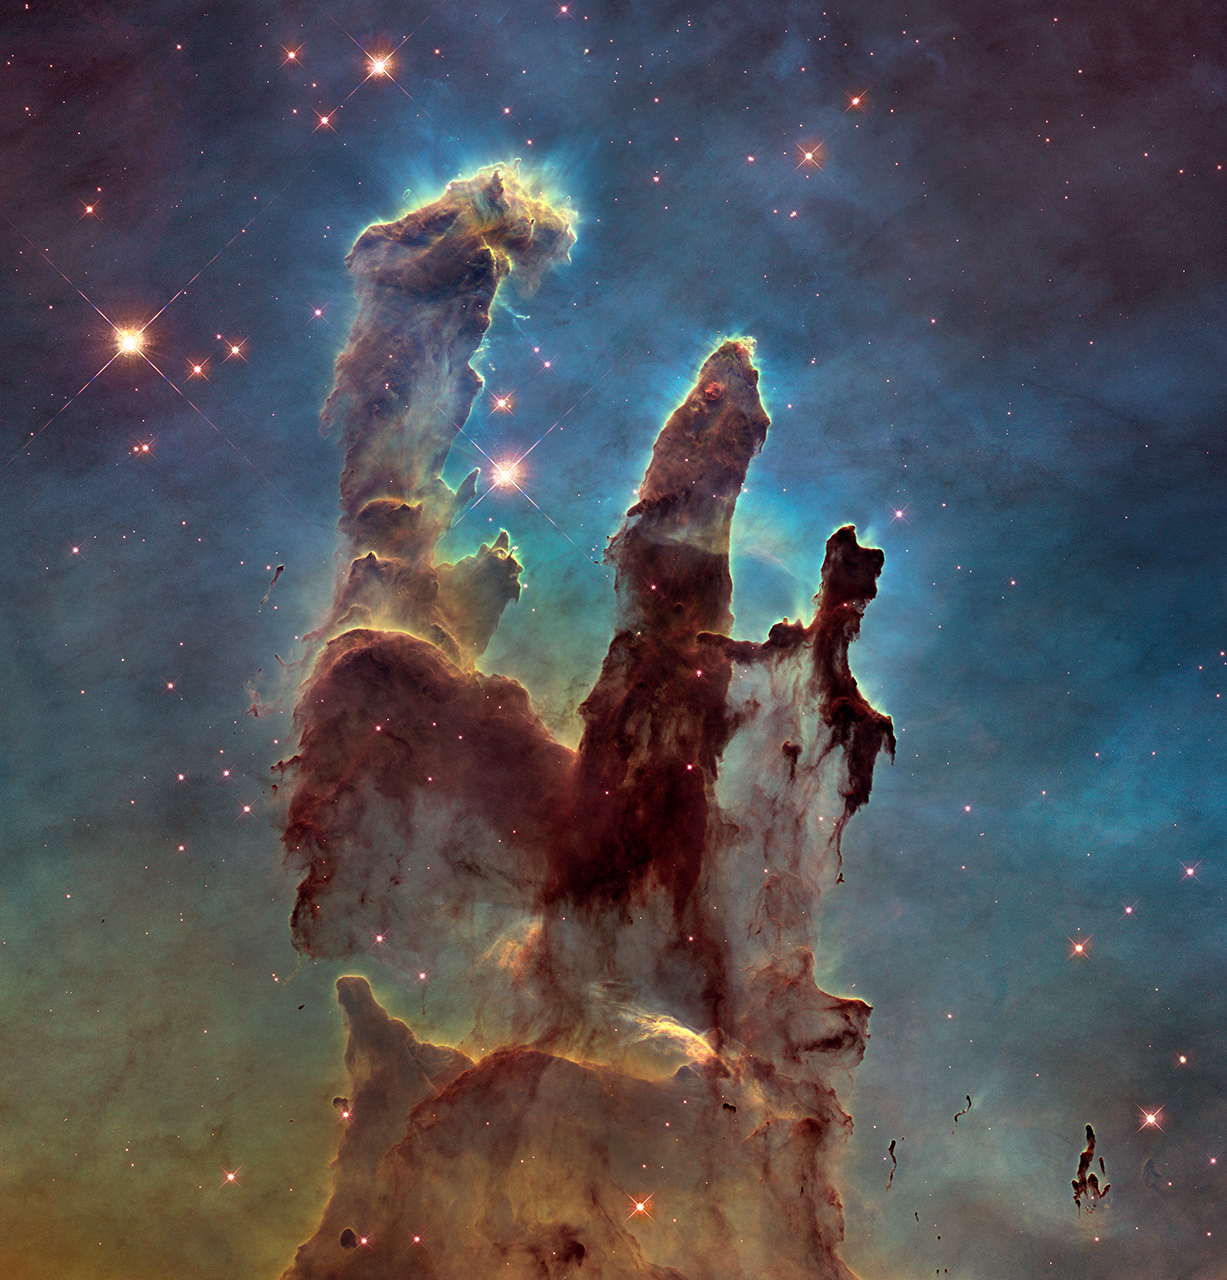
\includegraphics[width=\textwidth]{gtx_exp/space}
	\end{subfigure}~
	\begin{subfigure}[b]{0.32\textwidth}
		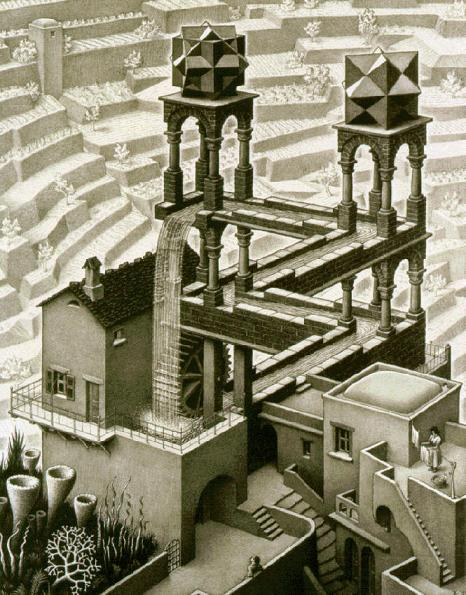
\includegraphics[width=\textwidth]{gtx_exp/waterfall}
	\end{subfigure}

	\begin{subfigure}[b]{0.32\textwidth}
		
\includegraphics[width=\textwidth]{gtx_exp/nips_logo_bin}
		\caption{logo}
	\end{subfigure}~
	\begin{subfigure}[b]{0.32\textwidth}
		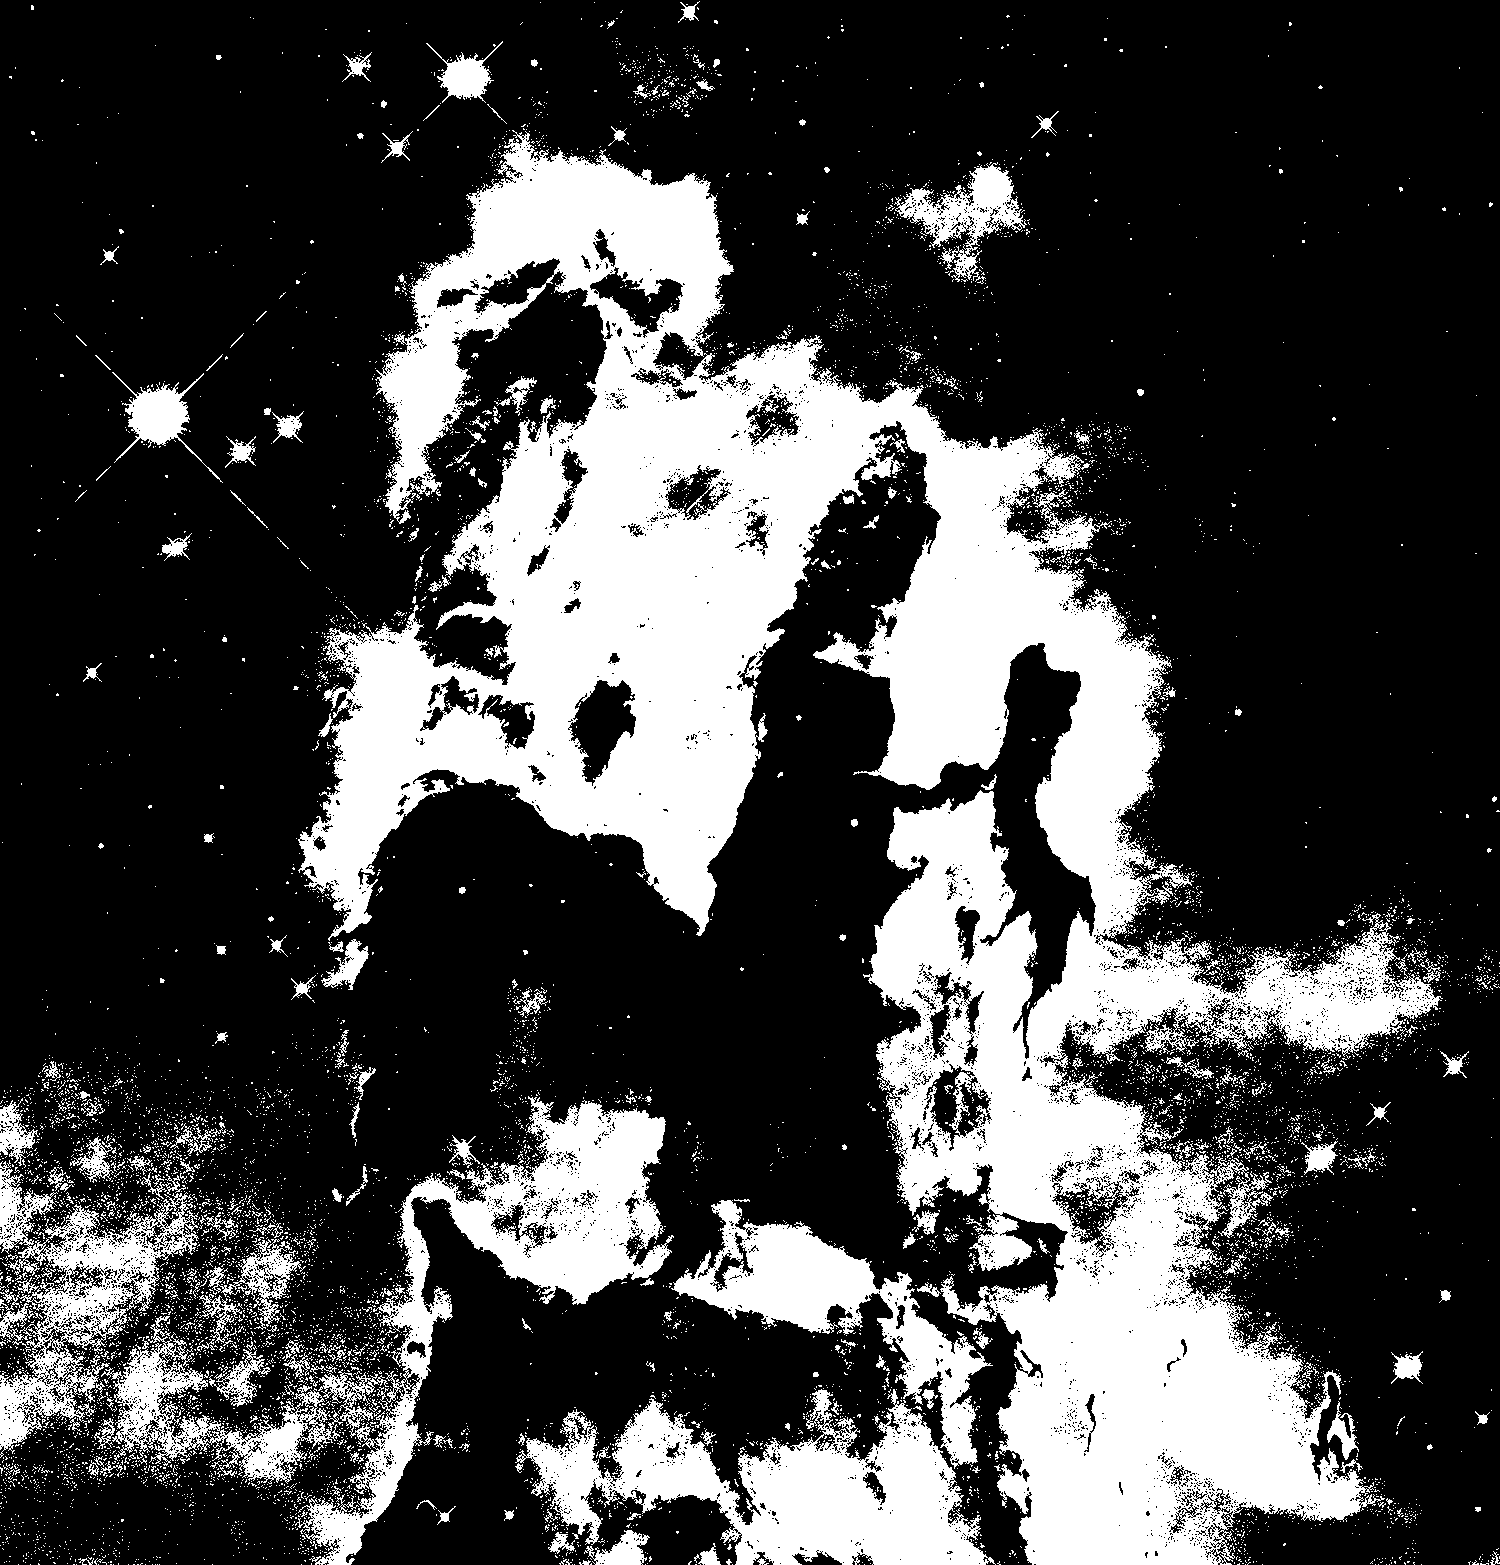
\includegraphics[width=\textwidth]{gtx_exp/space_bin}
		\caption{space}
	\end{subfigure}~
	\begin{subfigure}[b]{0.32\textwidth}
		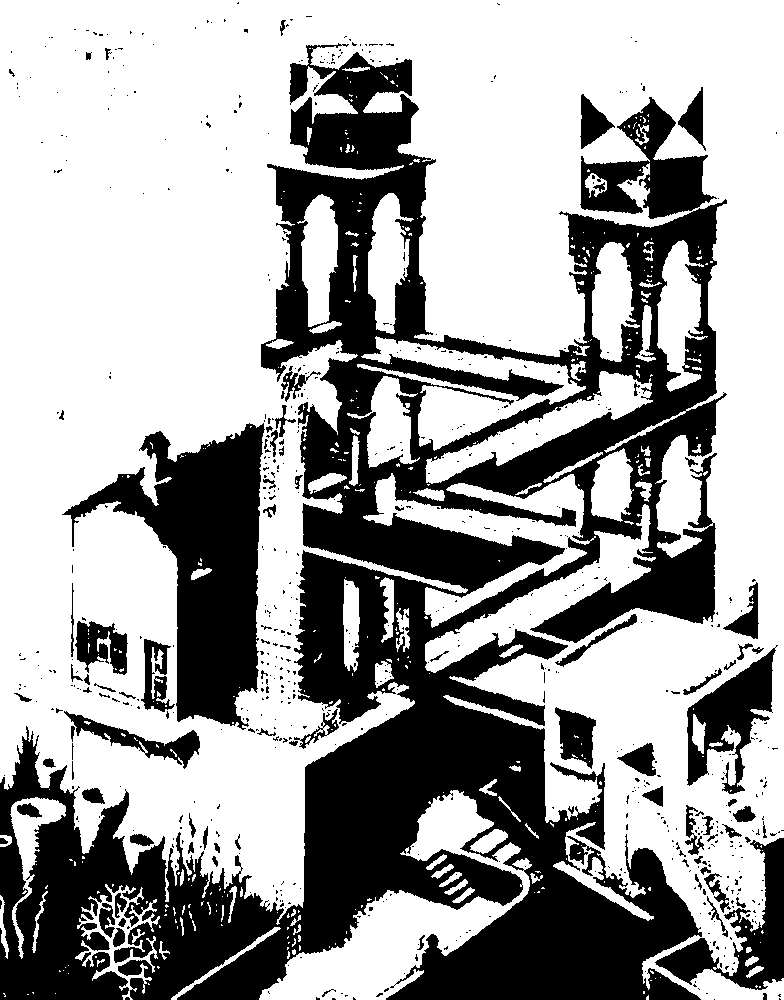
\includegraphics[width=\textwidth]{gtx_exp/waterfall_bin}
		\caption{waterfall}
	\end{subfigure}
	\caption{Real world pictures and their binarized version}\label{fig:gtx_xp_bwpics}
\end{figure}

\subsubsection{Stretch}

The first property of Galaxy trees we wish to evaluate is their stretch, which depends only of graph
topology. Recall that following equation~\autoref{eq:test_stretch_def}, we define the average test
edge stretch as $\frac{1}{|\etest{}|} \sum_{(u,v) \in \etest{}} |\mathrm{path}^T_{u,v}|$,
where $|\mathrm{path}^T_{u,v}|$ is the unique path between $u$ and $v$ in $T$.

As we consider unweighted graphs, we compare \gtx{} with a natural baseline, namely a spanning tree
rooted at the highest degree node and obtained through a breadth first visit of the graph. This
involves randomness in the order in which nodes are visited. Likewise in \gtx{}, the choice of the edge
linking two stars is not always unique, meaning that we have to break ties at random.  Therefore,
for each graph, we repeat the tree construction \np{12} times and present the average result, noting that
the variance (showed as error bar in \autoref{fig:gtx_xp_st}) is small.

On \lpa{} and \triangle{}, we see in \autoref{fig:gtx_xp_st} that both trees exhibits logarithmic stretch, although with a
larger constant for \gtx{}. Note that this is also the case for others low stretch tree methods
\autocite[Section 5.3.1]{papplow}. On \grid{} however, \gtx{} preserves this logarithmic stretch growth
while this is visually no longer the case for \bfs{}.
In that case, we cannot expect a better stretch than $\frac{\log n}{2048}$ according to
\autocite[Theorem 6.6]{LowerBound95}.

\begin{figure}[tbh]
	\centering
	\begin{subfigure}[b]{0.9\textwidth}
		\includegraphics[width=\textwidth]{gtx_exp/gridst}
		\caption{\grid{} }\label{fig:gtx_xp_gridst}
	\end{subfigure}

	\begin{subfigure}[b]{0.9\textwidth}
		\includegraphics[width=\textwidth]{gtx_exp/past}
		\caption{\lpa{} }\label{fig:gtx_xp_past}
	\end{subfigure}

	\begin{subfigure}[b]{0.9\textwidth}
		\includegraphics[width=\textwidth]{gtx_exp/trst}
		\caption{\triangle{} }\label{fig:gtx_xp_trst}
	\end{subfigure}
	\caption{Stretch over graphs of increasing size}\label{fig:gtx_xp_st}
\end{figure}

\subsubsection{Sign prediction}

The second design goal of Galaxy trees is to accurately predict the sign of edges in $\etest{}$.
Except for the three real datasets that already include signs\footnote{We nonetheless perform some
preprocessing in order to make them undirected and to remove the small proportion of conflicting edges
(e.g. positive from $u$ to $v$ but negative from $v$ to $u$).}, all the other are constructed,
meaning we have to set sign on their edges in the first place. This is done by partitioning the
nodes into two clusters. For \gplus{} we use node gender, for pictures we use node color (black or
white), and for all others, we propagate labels $0$ and $1$ from randomly selected high degree nodes.
Once each node belongs to one of the two clusters, we set the sign of an edge between two nodes to
be $+$ if they are in the same cluster and $-$ otherwise.  Predicting using path parity will thus
gives perfect result. To test performance in real situations, we then add noise, that
is we select a fraction of edges uniformly at random and flip their sign. 

Like in \autoref{s:exp}, we evaluate the performance of our prediction using the Matthews
Correlation Coefficient (MCC), defined in equation~\autoref{eq:troll_mcc} \vpageref{eq:troll_mcc}.
As showed in \autoref{fig:gtx_xp_mcc}, when the noise level is low, \gtx{} performs better than
\bfs{}. As the noise level gets higher, they have similar performance. Note also than in
\autoref{fig:gtx_xp_pasynthmcc}, \gtx{} is less sensible to the size of the graph.

\begin{figure}[tbh]
	\centering
	\begin{subfigure}[b]{0.47\textwidth}
		\includegraphics[width=\textwidth]{gtx_exp/grsynthmcc}
		\caption{Synthetic \grid{} }\label{fig:gtx_xp_grsynthmcc}
	\end{subfigure}~
	\begin{subfigure}[b]{0.47\textwidth}
		\includegraphics[width=\textwidth]{gtx_exp/grrwmcc}
		\caption{Pictures \grid{} }\label{fig:gtx_xp_grrwmcc}
	\end{subfigure}
	\begin{subfigure}[b]{0.47\textwidth}
		\includegraphics[width=\textwidth]{gtx_exp/pasynthmcc}
		\caption{Synthetic \lpa{} }\label{fig:gtx_xp_pasynthmcc}
	\end{subfigure}~
	\begin{subfigure}[b]{0.47\textwidth}
		\includegraphics[width=\textwidth]{gtx_exp/trmcc}
		\caption{\triangle{} }\label{fig:gtx_xp_trmcc}
	\end{subfigure}
	\begin{subfigure}[b]{0.47\textwidth}
		\includegraphics[width=\textwidth]{gtx_exp/parwmcc}
		\caption{Real world network }\label{fig:gtx_xp_parwmcc}
	\end{subfigure}
	\caption{MCC over various graphs}\label{fig:gtx_xp_mcc}
\end{figure}

To further assess the quality of our trees, we plug them in them into an existing heuristic method
to predict edge sign: \asym{}~\autocite{Kunegis2009}.
%\Todo{It might also be interesting to see if that would be a good training set for our troll method, although it has to be checked it makes sense from a running time point of view.}
It computes the exponential of the adjacency matrix after it has
been reduce to $z$ dimension. This allows to count the sign of all paths between two pairs of nodes
with decreasing weight depending of their length. To simulate an active learning setting, we reveal
only a subset of edge in $A$. This subset can be: $i)$ the edges forming a \bfs{}, $ii)$ the edges
forming a \gtx{} $iii)$ $|V|-1$ edges chosen uniformly at random.
We set the parameter $z$ equal to $15$ because $i)$ it is one of the best in \cite[Fig.
11]{Kunegis2009} and $ii)$ it performs well on real datasets in \cite[Fig.3]{Cesa-Bianchi2012a}.
% , and $iii)$ it was good in our initial testing (\texttt{20150401\_wed\_spectral.ipynb}).

As the \asym{} has a $O(n^3)$ complexity and uses quite some memory at prediction time, the larger
graphs used previously are not all included. The conclusion of \autoref{fig:gtx_xp_asym} is that
except on social networks, it is better to use spanning trees than random edges. Specifically, \gtx{}
on \grid{} and \bfs{} elsewhere.

\begin{figure}[tbh]
	\centering
	\begin{subfigure}[b]{0.47\textwidth}
		\includegraphics[width=\textwidth]{gtx_exp/grsynthasym}
		\caption{Synthetic \grid{} \label{fig:gtx_xp_grsynthasym}}
	\end{subfigure}~
	\begin{subfigure}[b]{0.47\textwidth}
		\includegraphics[width=\textwidth]{gtx_exp/grrwasym}
		\caption{\enquote{Real} \grid{} }\label{fig:gtx_xp_grrwasym}
	\end{subfigure}
	\begin{subfigure}[b]{0.47\textwidth}
		\includegraphics[width=\textwidth]{gtx_exp/pasynthasym}
		\caption{Synthetic \lpa{} }\label{fig:gtx_xp_pasynthasym}
	\end{subfigure}~
	\begin{subfigure}[b]{0.47\textwidth}
		\includegraphics[width=\textwidth]{gtx_exp/trasym}
		\caption{\triangle{} }\label{fig:gtx_xp_trasym}
	\end{subfigure}
	\begin{subfigure}[b]{0.47\textwidth}
		\includegraphics[width=\textwidth]{gtx_exp/parwasym}
		\caption{Real world network }\label{fig:gtx_xp_parwasym}
	\end{subfigure}
	\caption{\asym{} over various graphs}\label{fig:gtx_xp_asym}
\end{figure}

\iffalse
Finally\marginpars{Actually I never did it because \shz{} wasn't implemented at the time, so now is
a good occasion}\todo*{Run shazoo on galaxy tree} we also compare \gtx{} with \bfs{} and \rst{} on
the task of nodes prediction using \shz{} algorithm~\autocite{Vitale2012}.
\fi

